%--------------A VOTRE ATTENTION-------------%
% Les étudiants  qui disposent de plus de 3 chapitres dans leurs travaux peuvent en complèter
% Les Membres doivent figurer dans la dernière version finale du mémoire pour dépôt de mémoire

\newcommand{\lang}{1}

\ifnum\lang=1
    \documentclass{iid}
\else
    \documentclass{iidEn}
\fi

\usepackage{titletoc}
\setlength{\glsdescwidth}{0.65\textwidth}
% \usepackage{lscape}

\ifnum\lang=1
    \typeMemoire{Diplôme d’Ingénieur d'État }
\optionFormation{\textbf{Informatique et Ingénierie des Données}\\ 
\includegraphics[scale=0.08]{images/logoIID.png}}
\etudiant{Ziyad \textbf{RAKIB}}
\titreDuMemoire{Participation à la migration d'une architecture monolithique à une architecture microservices} 
\dateSoutenance{15/06/2023}
%\promo{2\up{ème}}
\anneeScolaire{\the\year}


%%maitre de mémoire
\encadrants{Abdelghani \textbf{Ghazdali} (interne)\\Nidal \textbf{Lamghari} (interne)\\ Bilal \textbf{Slayki} (externe)}

%% Membres du Jury
\jurys{%
\begin{tabular}{lll}
	OURDOU Amal &  Entité & Président \\
	OUMMI Hssaine & Entité & Examinateur
\end{tabular}	
}
\else
    \thesisType{State engineer diploma}
\formationOption{\textbf{Computer Science and Data Engineering}\\ 
\includegraphics[scale=0.08]{images/logoIID.png}}
\student{Ziyad \textbf{RAKIB}}
\thesisTitle{Participation in the migration from a monolithic architecture to a microservices architecture} 
\dateOfDefense{15/06/2023}
%\promo{2\up{ème}}
\schoolYear{\the\year}


%%maitre de mémoire
\tutors{Abdelghani \textbf{Ghazdali}\\Nidal \textbf{Lamghari}}

%% Membres du Jury
\jurys{%
\begin{tabular}{lll}
	Chairman's surname and first name          &  Entity & Chairman \\
	Surname and first name of the examiner     &  Entity & Examiner \\
	Surname and first name of the reporter     &  Entity & Reporter \\
	Surname and first name of the reporter     &  Entity & Reporter \\
\end{tabular}	
}
\fi


\hypersetup{
 pdftitle={--},
 pdfauthor={--},
 pdfsubject={--},
 pdfkeywords={--} 
 }

\color{bookColor}

%importation du glossaire
\loadglsentries{glossaire_reduit}

\begin{document}




\pageDeGarde%\pageTitre

\pagecolor{white}

%% page vide
\thispagestyle{empty}\ \clearpage
% ehrig2006graph
\newpage
% sommaire
\pagenumbering{roman}

\setcounter{tocdepth}{0}
\startlist{toc}
\printlist{toc}{}{\chapter*{Sommaire}}
\setcounter{tocdepth}{5}

\ifnum\lang=1
    %% rdedicaces
    \dedicace

\begin{fquote}
\begin{center}
\large{

\uppercase{à} mLorem ipsum dolor sit amet, consectetur adipiscing elit. Proin posuere euismod neque, non semper nibh viverra sed. Praesent ut varius magna. Fusce ipsum ante, semper nec interdum at, semper et lacus. Nulla ultrices magna a fringilla finibus,\\[12pt]
\uppercase{à} Lorem ipsum dolor sit amet, consectetur adipiscing elit. Proin posuere euismod neque, non semper nibh viverra sed. Praesent ut varius magna. Fusce ipsum ante, semper nec interdum at, semper et lacus. Nulla ultrices magna a fringilla finibus,\\[12pt]
\uppercase{à} Lorem ipsum dolor sit amet, consectetur adipiscing elit. Proin posuere euismod neque, non semper nibh viverra sed. Praesent ut varius magna. Fusce ipsum ante, semper nec interdum at, semper et lacus. Nulla ultrices magna a fringilla finibus,\\[12pt]
\uppercase{à} tous ceux qui me sont chers, à vous tous\\[12pt]
Merci.
}
\end{center}
\bigskip
\medskip
\end{fquote}

\begin{adjustwidth}{2cm}{1cm}
\hspace*{\fill} \textbf{\textit{\large{- Abdelghani}}}
\end{adjustwidth}

\clearpage

    \newpage 

    %% remerciements
    \remerciements

Tout d’abord, je remercie le grand Dieu puissant de nous donné la puissance pour continuer et dépasser toutes les difficultés.

\medskip

J’adresse mes remerciements à, \textbf{\LR{\large{Monsieur Abdelghani Ghazdali}}}, chef de filière Informatique et Ingénierie des Données qui a su assurer le bon déroulement des séances d’encadrement du début à la fin.

\medskip

Je tiens également à adresser mes sincères remerciements à \textbf{\LR{\large{Professeur Nidal Lamghari}}}, pour ses précieux conseils, son expertise et sa disponibilité tout au long de cette expérience. Votre encadrement attentionné m'a permis d'approfondir mes connaissances et de progresser dans mes compétences techniques. Je suis reconnaissant d'avoir pu bénéficier de votre expertise et de votre soutien constant.

\medskip

Au terme de ce travail, je tiens également à exprimer mes sincères remerciements et ma gratitude envers tous ceux qui, par leur enseignement, par leur soutien et leurs conseils, ont contribué au déroulement de ce projet.

\medskip
Par ailleurs, je tiens à exprimer ma gratitude envers \textbf{\LR{\large{IZICAP}}}, où j'ai eu la chance de réaliser mon projet de fin d'études. Je suis reconnaissant envers toute l'équipe de \textbf{\LR{\large{IZICAP}}} pour m'avoir accueilli chaleureusement et pour m'avoir permis de mettre en pratique mes connaissances académiques dans un environnement professionnel. Votre expertise, votre mentorat et vos ressources ont été d'une valeur inestimable pour la réalisation de ce projet.

\medskip

Je tiens à remercier spécialement \textbf{\LR{\large{M. Bilal SLAYKI}}}, mon encadrant en entreprise, pour son soutien constant, ses orientations judicieuses et son accompagnement précieux tout au long de ce projet. Votre expérience, vos conseils éclairés et votre bienveillance m'ont inspiré et ont grandement contribué à ma croissance professionnelle. Je vous suis reconnaissant d'avoir partagé votre expertise avec moi et d'avoir été un mentor exceptionnel.

\medskip

Finalement, mes remerciements s’adressent aussi à l’ensemble du corps professoral et administratif de l’ENSA Khouribga pour l’effort qu’ils fournissent afin de nous garantir une bonne formation et à l’équipe administrative et technique pour tous les services offerts.
    \newpage

    % Résume
    \resume
%\selectlanguage{french}






Ce rapport fournit une analyse approfondie du projet complexe entrepris pour faire évoluer la source de données de Izicap. Le projet a nécessité la suppression de MariaDB et la mise en place de Delta Lake, une solution de stockage et de traitement de données hautes performances. De plus, l'architecture monolithique existante a été divisée en microservices utilisant Spring Boot comme backend avec un connecteur approprié pour Delta Lake, et les micro-frontends ReactJS comme frontend.

\medskip

Le projet présentait de nombreux défis qui nécessitaient l'application de technologies et de stratégies avancées. Celles-ci comprenaient la migration des données, la garantie de la cohérence et de l'exactitude des données, la gestion de la complexité des systèmes distribués et l'intégration de diverses technologies et services. Le rapport décrit les différentes solutions développées pour relever ces défis, notamment l'utilisation d'algorithmes de traitement de données avancés, d'architectures informatiques distribuées et de la conteneurisation.

\medskip

Malgré les défis rencontrés, le projet reste un travail en cours. Le rapport donne un aperçu des efforts en cours pour améliorer l'évolutivité, les performances et la fonctionnalité globale du projet.

\vspace{1cm}


\noindent\rule[2pt]{\textwidth}{0.5pt}

{\textbf{Mots clés :}}
Projet, Source de données, Delta Lake, Monolith, Microservice, Spring Boot, ReactJS, Micro-Frontend, Back-End, Front-End, Données, Évolutivité, Performance.
\\
\noindent\rule[2pt]{\textwidth}{0.5pt}

\clearpage


    \newpage

    % Résume
    \resumeAn
%\begin{abstract}
This final year project report highlights the different stages of our project to transform a Groovy-based monolithic architecture into a Java-based microservices architecture, while transitioning from AngularJS to React and adopting a microfrontend approach. Our goal was to enhance the flexibility, maintainability, performance, data consistency, and modularity of our application.
\medskip

Initially, our codebase was developed as a monolith using Groovy. The first step of our project involved analyzing the monolithic architecture and identifying components that could be isolated into independent microservices. Concurrently, we evaluated the benefits of migrating from the outdated AngularJS framework to the more modern and performant React framework.

\medskip
We proceeded with the design and implementation of these microservices using Spring Boot, ensuring loose coupling between functionalities and effective communication among services. Simultaneously, we gradually migrated our AngularJS code to React, rewriting existing features according to React's best development practices.  
\medskip

To ensure data consistency among microservices, we implemented Delta Lake, an incremental data management technology. Delta Lake guaranteed reliable data and simplified secure read and write operations between services. Java connectors facilitated communication between the React-based frontend and Delta Lake, ensuring robust and secure connectivity. These connectors also enabled efficient read and write operations, ensuring data integrity and consistency.

\medskip
In parallel, we adopted a microfrontend approach for our frontend architecture, decoupling frontend features into autonomous modules. This provided greater flexibility and the ability to develop and deploy modules independently.

\medskip

Finally, to facilitate deployment and management of our microservices, React, and microfrontend architecture, we adopted Kubernetes and Docker. These tools enabled efficient orchestration, scaling of services, and simplified deployment across different environments.
\medskip

In conclusion, our project resulted in significant improvements in flexibility, maintainability, performance, data consistency, and modularity of our application. The transition from a Groovy-based monolithic architecture to a Java-based microservices architecture, combined with the migration from AngularJS to React, the adoption of Delta Lake, Java connectors, microfrontend, Kubernetes, and Docker, collectively optimized our system.

    \noindent\rule[2pt]{\textwidth}{0.5pt}
    {\textbf{Mots-clés :}}
    Monolithique, Groovy, Microservices, AngularJS, React, Delta Lake, Microfrontend, Kubernetes, Docker\\
    \noindent\rule[2pt]{\textwidth}{0.5pt}
\clearpage
    \newpage

    % Résume
    %\resumeAr
\setcode{utf8}

\chapter*{\hfill \RL{ملخص}}




\setstretch{1.3}
\begin{flushright}
\RL{
 في هذا التقرير، وردت إشارة إلى تنفيذ نظام كشف الوجه. والهدف من ذلك هو الكشف عن وجوه الناس المهتمين في منشور
  معين.
لقد إستعملنا لهذا الغرض لوحة الكترونية \LR{Raspberry pi 2} بالإضافة إلى وحدة الكاميرا الخاصة بها لملاحقة الوجوه و العين.
يستخدم  تطبيق كشف الوجه  خوارزمية قوية  لفيولا جونز مع  تدريب المصنف للكشف عن الوجه الإنساني والعينين، عن طريق اختيار أفضل مصنف ممكن.
سيتم حفظ البيانات لكل إعلان في قاعدة بيانات \LR{MySQL} . وقد تم إنشاء تطبيق ويب لهذا الغرض والذي سيمكن المستخدم من   
معرفة عدد الأشخاص  والمدة الإجمالية للمشاهدة في الفترة (ساعة، يوم، شهر )  على شكل رسم بياني.
}
\end{flushright}


\vspace{1cm}


\noindent\rule[2pt]{\textwidth}{0.5pt}
\begin{flushright}
\RL{\textbf{
كلمات مفتاحية \LR{:} } ك ك  
}

\end{flushright}
\noindent\rule[2pt]{\textwidth}{0.5pt}

%\end{abstract}







    \newpage

    \selectlanguage{french}
\else
    %% rdedicaces
    \dedicace

\begin{fquote}
\begin{center}
\large{

\uppercase{To} my mother, who showered me with her support and devoted me with unconditional love. You are for me an example of courage and continuous sacrifice. May this humble work bear witness to my affection, my eternal attachment and may it call upon me your continual blessing,\\[12pt]
\uppercase{To} my father, no dedication can express the love, esteem, devotion, and respect I have always had for you. Nothing in the world is worth the efforts made day and night for my education and my well-being. This work is the fruit of your sacrifices that you made for my education and training,\\[12pt]
\uppercase{To} my dear brothers, thank you for your love, support, and encouragement,\\[12pt]
\uppercase{To} all my dear friends, for the support you have given me, I say\\[12pt]
Thank you.
}
\end{center}
\bigskip
\medskip
\end{fquote}

\begin{adjustwidth}{2cm}{1cm}
\hspace*{\fill} \textbf{\textit{\large{- Ziyad}}}
\end{adjustwidth}

\clearpage

    \newpage 

    %% remerciements
    \remerciements

First and foremost, I would like to thank the Almighty Allah for granting us the strength to persevere and overcome all difficulties.

\medskip

I would like to express my gratitude to \textbf{\LR{\large{Mr.Abdelghani Ghazdali}}}, the head of the Computer Science and Data Engineering department, who ensured the smooth progress of the supervision sessions from start to finish.

\medskip

I would also like to extend my sincere thanks to \textbf{\LR{\large{Professor Nidal Lamghari}}}, for his valuable advice, expertise, and availability throughout this experience. Your attentive guidance allowed me to deepen my knowledge and improve my technical skills. I am grateful for the opportunity to benefit from your expertise and constant support.

\medskip

At the conclusion of this work, I would also like to express my sincere thanks and gratitude to all those who, through their teaching, support, and advice, contributed to the progress of this project.

\medskip

Furthermore, I would like to express my gratitude to \textbf{\LR{\large{IZICAP}}}, where I had the opportunity to carry out my final year project. I am grateful to the entire \textbf{\LR{\large{IZICAP}}} team for welcoming me warmly and allowing me to apply my academic knowledge in a professional environment. Your expertise, mentorship, and resources have been invaluable in the completion of this project.

\medskip

I would like to give special thanks to \textbf{\LR{\large{Mr.Bilal SLAYKI}}}, my supervisor in the company, for his constant support, wise guidance, and invaluable assistance throughout this project. Your experience, insightful advice, and kindness have inspired me and greatly contributed to my professional growth. I am grateful for sharing your expertise with me and for being an exceptional mentor.

\medskip

Finally, my thanks also go to the entire faculty and administrative staff of ENSA Khouribga for their efforts in providing us with a quality education, as well as the administrative and technical team for all the services provided.
    \newpage

    % Résume
    \resume
%\selectlanguage{french}






Ce rapport fournit une analyse approfondie du projet complexe entrepris pour faire évoluer la source de données de Izicap. Le projet a nécessité la suppression de MariaDB et la mise en place de Delta Lake, une solution de stockage et de traitement de données hautes performances. De plus, l'architecture monolithique existante a été divisée en microservices utilisant Spring Boot comme backend avec un connecteur approprié pour Delta Lake, et les micro-frontends ReactJS comme frontend.

\medskip

Le projet présentait de nombreux défis qui nécessitaient l'application de technologies et de stratégies avancées. Celles-ci comprenaient la migration des données, la garantie de la cohérence et de l'exactitude des données, la gestion de la complexité des systèmes distribués et l'intégration de diverses technologies et services. Le rapport décrit les différentes solutions développées pour relever ces défis, notamment l'utilisation d'algorithmes de traitement de données avancés, d'architectures informatiques distribuées et de la conteneurisation.

\medskip

Malgré les défis rencontrés, le projet reste un travail en cours. Le rapport donne un aperçu des efforts en cours pour améliorer l'évolutivité, les performances et la fonctionnalité globale du projet.

\vspace{1cm}


\noindent\rule[2pt]{\textwidth}{0.5pt}

{\textbf{Mots clés :}}
Projet, Source de données, Delta Lake, Monolith, Microservice, Spring Boot, ReactJS, Micro-Frontend, Back-End, Front-End, Données, Évolutivité, Performance.
\\
\noindent\rule[2pt]{\textwidth}{0.5pt}

\clearpage


    \newpage

    % Résume
    \resumeAn
%\begin{abstract}
This final year project report highlights the different stages of our project to transform a Groovy-based monolithic architecture into a Java-based microservices architecture, while transitioning from AngularJS to React and adopting a microfrontend approach. Our goal was to enhance the flexibility, maintainability, performance, data consistency, and modularity of our application.
\medskip

Initially, our codebase was developed as a monolith using Groovy. The first step of our project involved analyzing the monolithic architecture and identifying components that could be isolated into independent microservices. Concurrently, we evaluated the benefits of migrating from the outdated AngularJS framework to the more modern and performant React framework.

\medskip
We proceeded with the design and implementation of these microservices using Spring Boot, ensuring loose coupling between functionalities and effective communication among services. Simultaneously, we gradually migrated our AngularJS code to React, rewriting existing features according to React's best development practices.  
\medskip

To ensure data consistency among microservices, we implemented Delta Lake, an incremental data management technology. Delta Lake guaranteed reliable data and simplified secure read and write operations between services. Java connectors facilitated communication between the React-based frontend and Delta Lake, ensuring robust and secure connectivity. These connectors also enabled efficient read and write operations, ensuring data integrity and consistency.

\medskip
In parallel, we adopted a microfrontend approach for our frontend architecture, decoupling frontend features into autonomous modules. This provided greater flexibility and the ability to develop and deploy modules independently.

\medskip

Finally, to facilitate deployment and management of our microservices, React, and microfrontend architecture, we adopted Kubernetes and Docker. These tools enabled efficient orchestration, scaling of services, and simplified deployment across different environments.
\medskip

In conclusion, our project resulted in significant improvements in flexibility, maintainability, performance, data consistency, and modularity of our application. The transition from a Groovy-based monolithic architecture to a Java-based microservices architecture, combined with the migration from AngularJS to React, the adoption of Delta Lake, Java connectors, microfrontend, Kubernetes, and Docker, collectively optimized our system.

    \noindent\rule[2pt]{\textwidth}{0.5pt}
    {\textbf{Mots-clés :}}
    Monolithique, Groovy, Microservices, AngularJS, React, Delta Lake, Microfrontend, Kubernetes, Docker\\
    \noindent\rule[2pt]{\textwidth}{0.5pt}
\clearpage
    \newpage

    % Résume
    %\resumeAr
\setcode{utf8}

\chapter*{\hfill \RL{ملخص}}




\setstretch{1.3}
\begin{flushright}
\RL{
 في هذا التقرير، وردت إشارة إلى تنفيذ نظام كشف الوجه. والهدف من ذلك هو الكشف عن وجوه الناس المهتمين في منشور
  معين.
لقد إستعملنا لهذا الغرض لوحة الكترونية \LR{Raspberry pi 2} بالإضافة إلى وحدة الكاميرا الخاصة بها لملاحقة الوجوه و العين.
يستخدم  تطبيق كشف الوجه  خوارزمية قوية  لفيولا جونز مع  تدريب المصنف للكشف عن الوجه الإنساني والعينين، عن طريق اختيار أفضل مصنف ممكن.
سيتم حفظ البيانات لكل إعلان في قاعدة بيانات \LR{MySQL} . وقد تم إنشاء تطبيق ويب لهذا الغرض والذي سيمكن المستخدم من   
معرفة عدد الأشخاص  والمدة الإجمالية للمشاهدة في الفترة (ساعة، يوم، شهر )  على شكل رسم بياني.
}
\end{flushright}


\vspace{1cm}


\noindent\rule[2pt]{\textwidth}{0.5pt}
\begin{flushright}
\RL{\textbf{
كلمات مفتاحية \LR{:} } ك ك  
}

\end{flushright}
\noindent\rule[2pt]{\textwidth}{0.5pt}

%\end{abstract}







    \newpage

    \selectlanguage{english}
\fi


\dominitoc% initializer les minitoc
\tableofcontents
\newpage

%liste des figures
\listoffigures 
\newpage

%liste des tableaux
\listoftables
\newpage

%%liste des algo
%\listofalgorithmes
%\newpage
%


%% Les sigles et acronymes
\listofsigle\begin{tabular}{rl}
API & Application programming interface \\
VSC & Visual Studio Code \\
DL & Delta Lake \\
REST & RepresEntational State Transfer \\
AWS & Amazon Web Services \\
GCP & Google Cloud Platform \\
AZR & Microsoft Azure \\
S3 & Simple Storage Service \\
IAM & Identity and Access Management \\
MinIO & Minimal Object Storage \\
SQL & Structured Query Language \\
DB & Database \\
ACID & Atomicity, Consistency, Isolation, Durability \\
OLTP & Online Transaction Processing \\
OLAP & Online Analytical Processing \\
ReactJS & React JavaScript \\
SPA & Single Page Application \\
JS & JavaScript \\
CSS & Cascading Style Sheets \\
HTML & Hypertext Markup Language \\
UI & User Interface \\
API & Application Programming Interface \\
Spark & Apache Spark \\
Hadoop & Apache Hadoop \\
HDFS & Hadoop Distributed File System \\
YARN & Yet Another Resource Negotiator \\
MapReduce & MapReduce Programming Model \\
Metadata & Data about Data \\
ETL & Extract, Transform, Load \\
ELT & Extract, Load, Transform \\
CRM & Customer Relationship Management \\
RDBMS & Relational Database Management System \\

\end{tabular}

\newpage

%% Les sigles et acronymes
%\setglossarystyle{altlist}
%\printglossary[title=Liste des acronymes, toctitle=Liste des acronymes, type=\acronymtype]
%\newpage

% Le glossaire proprement dit
%\setglossarystyle{super}
%\printglossary[type=main]


\pagenumbering{arabic}
\setcounter{page}{1}
%%introduction
\introduction
bla bla bla \gls{acro} puis \Gls{acroglo} et enfin \gls{glossaire}
%\lhead[]{} \rhead[]{} \chead[]{}
\ifnum\lang=1
    \selectlanguage{french}
\else
    \selectlanguage{english}
\fi
\fancyhead[L]{\tiny \leftmark}
\fancyhead[R]{\scriptsize \rightmark}
\fancyfoot[C]{\thepage}


\ifnum\lang=1
    \chapter{Contexte général du projet}\label{chap:1}
    \minitoc
\addcontentsline{toc}{section}{Introduction}
\section*{Introduction}

\section{About}
Izicap est un pionnier dans l'utilisation des données de cartes de paiement et les transforme en une connaissance client et des informations commerciales puissantes pour les commerçants, leur permettant de gérer leurs propres programmes de fidélité et campagnes de marketing numérique. 
Ces services marketing, fournis par les acquéreurs utilisant les solutions SaaS d'Izicap, redonnent rapidement de la croissance aux entreprises marchandes en renforçant les dépenses et la fidélité de leurs clients (les titulaires de carte). 
La solution innovante de CRM et de fidélité liée aux cartes d'Izicap donne aux acquéreurs un avantage concurrentiel en monétisant leurs données de transactions de paiement, en générant de nouvelles sources de revenus et en améliorant leurs capacités de rétention.
Après s'être solidement implanté en France grâce à des partenariats avec le Groupe BPCE et le Crédit Agricole, Izicap s'est associé à Nexi, le premier acquéreur et Fintech en Italie et a rejoint le programme StartPath de Mastercard dans le but d'étendre considérablement sa portée mondiale. 
Izicap s'associe aux principaux fournisseurs de solutions de paiement tels qu'Ingenico, Verifone, Poynt et PAX, et rend sa solution CRM et Fidélité liée à la carte disponible sur les terminaux de paiement les plus populaires et les plus innovantes.

\section{Organigramme}
informations sur Izicap

\addcontentsline{toc}{section}{Conclusion}
\section*{Conclusion}

    
    \chapter{Informatique décisionnelle et Choix de solutions}\label{chap:2}
    \addcontentsline{toc}{section}{Introduction}

\section*{Introduction}

L'informatique décisionnelle, également connue sous le terme de Business Intelligence (BI), englobe les processus, les technologies et les outils utilisés pour collecter, stocker, analyser et présenter les données dans le but de soutenir la prise de décision et d'aider les entreprises à obtenir des informations exploitables. L'informatique décisionnelle implique la transformation des données brutes en informations significatives et en connaissances exploitables pour les décideurs. On va voir dans ce chaptire pourquoi on a decidé d'opter pour Delta Lake au lieu de ses contre-parts.

\section{Différence entre un data warehouse, un data lake, un datalakehouse et un delta lake}
\begin{enumerate}
    \item[$\bullet$] \textbf{Data Warehouse:} Un data warehouse est une base de données centralisée qui est spécifiquement conçue pour le reporting et l'analyse. Il stocke les données structurées provenant de différentes sources, les organise selon un modèle de données prédéfini et les optimise pour des requêtes analytiques. Les données dans un data warehouse sont généralement cohérentes, intégrées et historisées. Cependant, la construction et la maintenance d'un data warehouse peuvent être complexes et coûteuses.
    \item[$\bullet$] \textbf{Data Lake:} Un data lake est un référentiel de données centralisé qui stocke de grandes quantités de données brutes, structurées et non structurées. Contrairement au data warehouse, le data lake ne nécessite pas une modélisation préalable des données. Il offre une grande flexibilité et évolutivité pour stocker des données hétérogènes. Cependant, l'intégration et la qualité des données peuvent être des défis dans un data lake.
    \item[$\bullet$] \textbf{Datalakehouse:} Le datalakehouse est une architecture émergente qui combine les avantages du data warehouse et du data lake. Il permet de stocker et de traiter à la fois des données brutes et des données structurées dans un environnement centralisé. Cette approche hybride offre la flexibilité d'un data lake et la capacité d'analyse d'un data warehouse. Cependant, la mise en place d'un datalakehouse peut nécessiter des efforts supplémentaires pour garantir la qualité des données et l'efficacité des requêtes.
    \item[$\bullet$] \textbf{Delta Lake:} Delta Lake est une technologie qui s'intègre aux data lakes existants pour fournir des fonctionnalités supplémentaires, telles que la gestion des transactions ACID (Atomicité, Cohérence, Isolation, Durabilité), la gestion des mises à jour incrémentielles et la garantie de la cohérence des données. Delta Lake est construit sur Apache Parquet et Apache Arrow, ce qui permet d'accélérer les requêtes analytiques et d'améliorer les performances globales. Cependant, l'utilisation de Delta Lake peut nécessiter des compétences techniques supplémentaires et peut avoir un impact sur la complexité de l'architecture de données. 
\end{enumerate}

% \subsection{Avantages et inconvénients de chaque architecture}

\subsection{Data Warehouse}
\textbf{Avanatges:}
\begin{enumerate}
    \item Données cohérentes et intégrées
    \item Modélisation préalable des données pour une analyse optimisée
    \item Hautes performances pour les requêtes analytiques
\end{enumerate}

\textbf{Inconvénients:}
\begin{enumerate}
    \item Coût élevé de construction et de maintenance
    \item Complexité de la modélisation des données
    \item Limitations pour l'intégration de données non structurées
\end{enumerate}

\subsection{Data Lake}
\textbf{Avanatges:}
\begin{enumerate}
    \item Stockage économique de grandes quantités de données
    \item Flexibilité pour intégrer des données brutes et non structurées
    \item Capacité à traiter des données de différentes sources
\end{enumerate}

\textbf{Inconvénients:}
\begin{enumerate}
    \item Difficulté à maintenir la qualité des données et la gouvernance
    \item Besoin d'outils avancés pour l'analyse et le traitement des données
    \item Requiert des compétences techniques pour l'exploitation efficace des données
\end{enumerate}

\subsection{Datalakehouse}
\textbf{Avanatges:}
\begin{enumerate}
    \item Combinaison des avantages du data warehouse et du data lake
    \item Flexibilité pour stocker et analyser des données brutes et structurées
    \item Possibilité d'évoluer en fonction des besoins évolutifs
\end{enumerate}

\textbf{Inconvénients:}
\begin{enumerate}
    \item Nécessite des efforts supplémentaires pour la qualité des données
    \item Complexité accrue de l'architecture de données
    \item Besoin de compétences techniques pour la mise en place et la gestion
\end{enumerate}

\subsection{Delta Lake (Datalakehouse)}
\textbf{Avanatges:}
\begin{enumerate}
    \item Gestion des transactions ACID pour une cohérence des données
    \item Prise en charge des mises à jour incrémentielles et du traitement des flux de données
    \item Hautes performances pour les requêtes analytiques
\end{enumerate}

\textbf{Inconvénients:}
\begin{enumerate}
    \item Nécessite des compétences techniques spécifiques
    \item Impact sur la complexité de l'architecture de données existante
    \item Peut nécessiter des adaptations pour une intégration transparente avec les outils existants
\end{enumerate}

\begin{figure}[H]
\centering
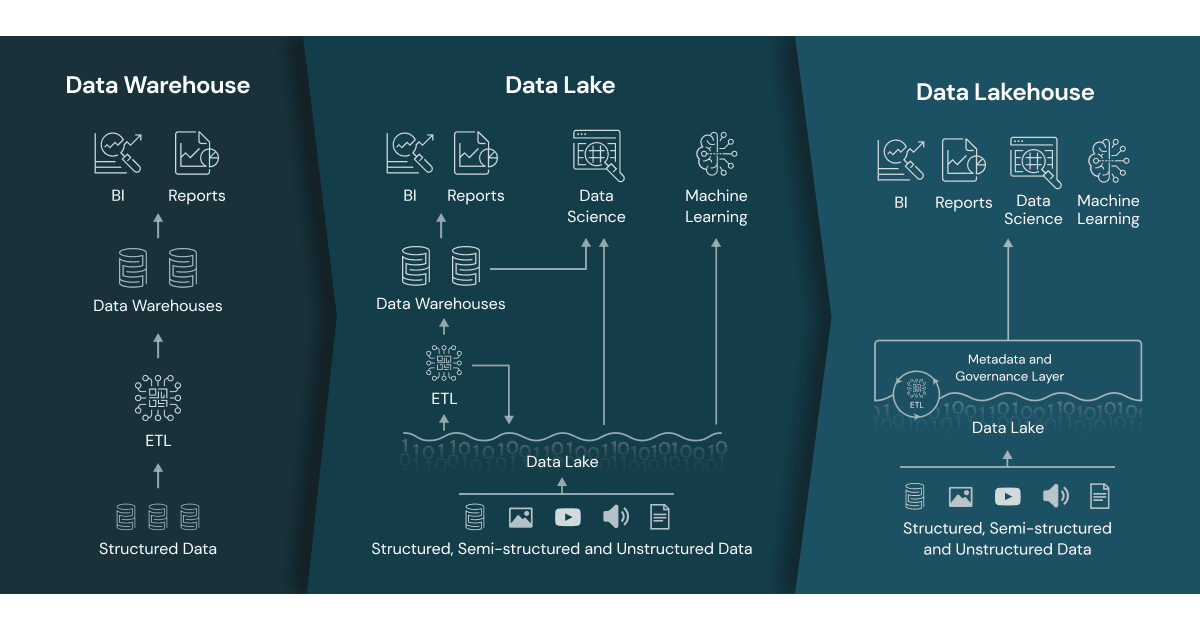
\includegraphics[width=\linewidth]{images/data-warehouse-data-lake-datalakehouse.png}
\caption{Data Warehouse vs Data Lake vs Data Lakehouse}\label{fig:data-warehouse-data-lake-datalakehouse}
\end{figure}

\section{Différence entre une architecture microservices et une architecture monolithique}
\begin{enumerate}
    \item[$\bullet$] \textbf{Monolithe:} un monolithe est une application qui est conçue comme une entité unique et indivisible. Toutes les fonctionnalités de l'application sont regroupées dans un seul code base, partageant les mêmes ressources, bases de données et déploiements. Dans une architecture monolithique, il n'y a pas de découpage clair des fonctionnalités en services indépendants. Toute modification ou évolution de l'application nécessite des changements au niveau global.
    \item[$\bullet$] \textbf{Microservice:} Un microservice est une approche architecturale dans laquelle une application est construite comme un ensemble de services indépendants et autonomes, chacun se concentrant sur une fonction spécifique de l'application. Chaque microservice est développé, déployé et géré de manière indépendante, ce qui permet une évolutivité, une flexibilité et une maintenance plus faciles. Les microservices communiquent entre eux via des interfaces bien définies, généralement basées sur des API REST ou des messages.
\end{enumerate}

\subsection{Avantages et Inconvénients de l'architecture monolithique}
\textbf{Avanatges:}
\begin{enumerate}
    \item \textbf{Simplicité de développement initial :} L'approche monolithique permet de développer rapidement une application en regroupant toutes les fonctionnalités dans un seul code base. Cela facilite la gestion des dépendances et la coordination des différentes parties de l'application.
    \item \textbf{Moins de complexité opérationnelle :} Avec une architecture monolithique, il y a moins de composants et de services à gérer, ce qui simplifie les opérations de déploiement, de surveillance et de gestion. Tout est regroupé au sein d'un seul déploiement, ce qui peut être plus facile à gérer pour les équipes opérationnelles.
    \item \textbf{Communications internes plus rapides :} Dans une architecture monolithique, les communications entre les différentes parties de l'application sont plus rapides car elles se font généralement via des appels de méthode internes. Cela peut être bénéfique en termes de performances et de latence réduite.
\end{enumerate}

\textbf{Inconvénients:}
\begin{enumerate}
    \item \textbf{Difficulté à faire évoluer et à maintenir:} Avec une architecture monolithique, les évolutions et les mises à jour peuvent être plus complexes, car chaque changement doit être effectué sur l'ensemble de l'application. Cela peut rendre le processus de développement plus lent et entraîner des risques d'erreurs lors des déploiements.
    \item \textbf{Rigidité technologique:} Une architecture monolithique peut entraîner une rigidité technologique, car toutes les parties de l'application doivent utiliser les mêmes technologies et langages de programmation. Cela peut limiter les possibilités d'adopter de nouvelles technologies ou de faire évoluer des parties spécifiques de l'application de manière indépendante.
    \item \textbf{Difficulté à isoler les problèmes:} En cas de problème ou de bug, il peut être plus difficile de les isoler et de les résoudre dans une architecture monolithique. Étant donné que toutes les fonctionnalités sont regroupées dans un seul code base, il peut être complexe de localiser l'origine exacte du problème.
    \item \textbf{Moins de flexibilité en termes d'évolutivité:} L'architecture monolithique peut poser des défis en termes d'évolutivité. Si une partie de l'application nécessite plus de ressources pour gérer une charge élevée, il peut être difficile d'ajuster cette partie spécifique sans augmenter les ressources globales de l'application.
\end{enumerate}

\subsection{Avantages et Inconvénients de l'architecture microservices}
\textbf{Avanatges:}
\begin{enumerate}
    \item \textbf{Scalabilité et évolutivité:} Les microservices permettent de découper l'application en plusieurs services autonomes et indépendants, ce qui facilite la scalabilité horizontale. Chaque microservice peut être déployé, mis à l'échelle et mis à jour indépendamment, ce qui permet de gérer efficacement les variations de charge et de garantir une évolutivité facile en fonction des besoins de l'entreprise.
    \item \textbf{Flexibilité technologique:} Les microservices offrent la possibilité d'utiliser différentes technologies et langages de programmation pour chaque service. Dans notre cas, l'utilisation de Spring Boot nous permet de profiter de son écosystème riche et de ses fonctionnalités avancées pour le développement rapide d'applications. Cela permet également d'adopter des technologies spécifiques en fonction des besoins de chaque microservice, favorisant ainsi la flexibilité technologique.
    \item \textbf{Indépendance et autonomie:} Chaque microservice est conçu pour fonctionner de manière autonome, ce qui permet une meilleure isolation des fonctionnalités et des responsabilités. Cela facilite la maintenance, le test et le déploiement des services de manière indépendante, réduisant ainsi les risques d'impact sur l'ensemble du système en cas de modifications ou de problèmes.
    \item \textbf{Développement et déploiement rapides:} Les microservices permettent une approche de développement agile en favorisant des cycles de développement plus courts. Les équipes peuvent se concentrer sur des fonctionnalités spécifiques et les développer de manière indépendante, ce qui accélère le développement global du système. De plus, les microservices peuvent être déployés de manière continue grâce à l'utilisation de techniques de déploiement automatisées, facilitant ainsi les mises à jour fréquentes et rapides.
    \item \textbf{Facilité de maintenance et de débogage:} En raison de leur nature modulaire, les microservices facilitent la maintenance et le débogage du système. En cas de problème ou d'erreur, il est plus facile d'identifier le service spécifique concerné et de résoudre le problème sans impacter l'ensemble du système.
\end{enumerate}

\textbf{Inconvénients:}
\begin{enumerate}
    \item \textbf{Complexité de la gestion des communications:} Les microservices impliquent une communication entre différents services, généralement via des API REST ou des messages. La gestion de ces communications peut devenir complexe, en particulier lorsque de nombreux services sont impliqués. Des problèmes tels que la latence, la cohérence des données et la gestion des erreurs peuvent se poser.
    \item \textbf{Surcharge de développement initial:} Le développement de microservices nécessite un effort supplémentaire pour découper correctement les fonctionnalités, définir les interfaces et mettre en place une infrastructure appropriée pour le déploiement et la communication des services. Cela peut augmenter la charge de travail initiale et nécessiter des compétences spécifiques en matière d'architecture distribuée.
    \item \textbf{Gestion de la cohérence des données:} Avec des microservices, chaque service peut avoir sa propre base de données ou son propre stockage de données. Cela peut rendre la gestion de la cohérence des données plus complexe, en particulier lorsqu'il y a des mises à jour simultanées impliquant plusieurs services. Des techniques telles que les transactions distribuées ou les événements asynchrones peuvent être nécessaires pour maintenir la cohérence des données.
    \item \textbf{Déploiement et gestion de plusieurs services:} Avec les microservices, il y a un nombre accru de services à déployer, gérer et surveiller. Cela peut nécessiter des compétences supplémentaires en matière d'automatisation des déploiements, de gestion des conteneurs ou de gestion des clusters. Le suivi des performances et du comportement de chaque service peut également devenir plus complexe.
    \item \textbf{Coût de l'infrastructure:} Les microservices peuvent nécessiter une infrastructure plus complexe et des ressources supplémentaires pour fonctionner efficacement. Chaque service doit être déployé et exécuté indépendamment, ce qui peut entraîner une augmentation des coûts liés aux ressources informatiques et à la gestion de l'infrastructure.
\end{enumerate}

\begin{figure}[H]
\centering
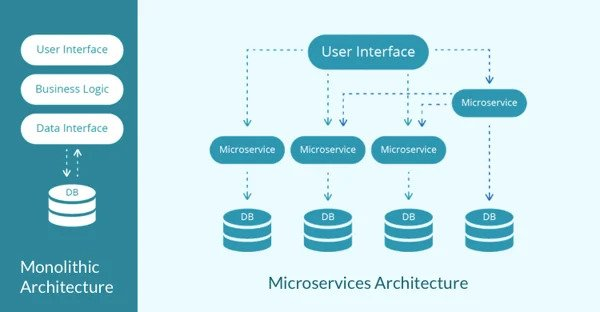
\includegraphics[width=0.6\linewidth]{images/monolithicvsmicroservice.jpg}
\caption{Architecture monolithique vs microservice}\label{fig:monolithevsmicroservice}
\end{figure}

\section{Différence entre une architecture microfrontends et une architecture monolithique fronend}
\begin{enumerate}
    \item[$\bullet$] \textbf{Monolithe frontend:} Un frontend monolithique est une approche architecturale où l'application frontend est développée comme une seule entité, généralement en utilisant un framework spécifique tel qu'AngularJS. Toutes les fonctionnalités, les vues et les logiques de l'interface utilisateur sont regroupées dans un seul code base.
    \item[$\bullet$] \textbf{Microfrontends:} Les microfrontends sont une approche architecturale où une application frontend est divisée en plusieurs micro-applications indépendantes, chacune étant responsable d'une partie spécifique de l'interface utilisateur. Chaque micro-application peut être développée, déployée et évoluée de manière autonome, utilisant différents frameworks, langages et technologies.
\end{enumerate}

\subsection{Avantages et Inconvénients du monolithe frontend}
\textbf{Avanatges:}
\begin{enumerate}
    \item \textbf{Simplicité de développement initial:} L'architecture monolithique avec AngularJS offre une approche simple pour le développement initial de l'application frontend. Toutes les fonctionnalités sont regroupées dans un seul code base, ce qui facilite la coordination et la gestion du développement.
    \item \textbf{Facilité de communication entre les composants:} Dans une architecture monolithique, les composants AngularJS peuvent communiquer entre eux facilement via le système de directives et de services d'AngularJS. Cela permet une communication rapide et efficace entre les différentes parties de l'application. 
    \item \textbf{Interopérabilité des fonctionnalités:} Étant donné que toutes les fonctionnalités sont développées en utilisant AngularJS, il est plus facile de partager des fonctionnalités et des modules entre les différentes parties de l'application. Cela favorise la réutilisation du code et simplifie la maintenance.
\end{enumerate}

\textbf{Inconvénients:}
\begin{enumerate}
    \item \textbf{Difficulté à maintenir et à faire évoluer:} À mesure que l'application frontend devient plus complexe, la maintenance et l'évolution de l'architecture monolithique avec AngularJS peuvent devenir difficiles. Les modifications apportées à une partie de l'application peuvent avoir des répercussions sur l'ensemble du code base, ce qui rend le processus de développement plus lent et risqué.
    \item \textbf{Limitations de performance:} Dans une architecture monolithique, toutes les fonctionnalités sont chargées en même temps, ce qui peut entraîner des problèmes de performance si l'application devient volumineuse. Les temps de chargement peuvent être plus longs et l'application peut être moins réactive pour l'utilisateur.
    \item \textbf{Flexibilité limitée:} L'architecture monolithique avec AngularJS peut limiter la flexibilité technologique. Étant donné que toutes les parties de l'application sont développées en utilisant AngularJS, il peut être difficile d'introduire de nouvelles technologies ou de faire évoluer certaines parties spécifiques de l'application de manière indépendante.
\end{enumerate}

\subsection{Avantages et Inconvénients de l'architecture microfrontends}
\textbf{Avanatges:}
\begin{enumerate}
    \item \textbf{Indépendance des équipes de développement:} Chaque micro-application peut être développée par une équipe distincte, ce qui favorise une plus grande autonomie et une meilleure collaboration entre les équipes de développement. Chaque équipe peut choisir les technologies qui conviennent le mieux à ses besoins.
    \item \textbf{Évolutivité et facilité de maintenance:} L'architecture microfrontends permet de faire évoluer et de maintenir les différentes parties de l'application de manière indépendante. Les modifications apportées à une micro-application n'ont pas d'impact sur les autres, ce qui facilite la maintenance et permet de déployer rapidement de nouvelles fonctionnalités.
    \item \textbf{Flexibilité technologique:} Chaque micro-application peut utiliser la technologie, le framework ou le langage de programmation qui convient le mieux à son domaine spécifique. Cela permet d'introduire de nouvelles technologies et d'exploiter les avantages des derniers développements dans le domaine de l'ingénierie logicielle.
\end{enumerate}

\textbf{Inconvénients:}
\begin{enumerate}
    \item \textbf{Complexité accrue:} L'architecture microfrontends introduit une certaine complexité dans le développement et le déploiement de l'application. La gestion des interactions et de la communication entre les différentes micro-applications peut nécessiter une planification et une coordination supplémentaires.
    \item \textbf{Coût de développement initial:} Le développement d'une architecture microfrontends peut nécessiter un investissement initial plus important en termes de ressources et de temps. Le développement de plusieurs micro-applications distinctes et la mise en place de l'infrastructure nécessaire peuvent être plus coûteux que le développement d'une application monolithique.
    \item \textbf{Surcharge réseau:} L'utilisation d'une architecture microfrontends peut entraîner une surcharge réseau plus importante, car chaque micro-application nécessite des requêtes et des chargements de ressources distincts. Cela peut avoir un impact sur les performances de l'application et nécessiter une gestion efficace du réseau.
\end{enumerate}

\begin{figure}[H]
\centering
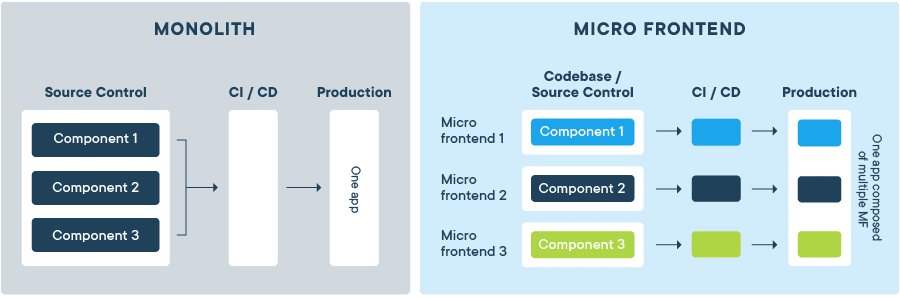
\includegraphics[width=\linewidth]{images/micro-frontend-vs-monolith-frontend.png}
\caption{Architecture monolithique frontend vs microfrontends}\label{fig:monolithfrontendvsmicrofrontends}
\end{figure}

\section{Cheminement de la solution}
\subsection{Partie Data}
Dans le cadre de notre solution, nous avons opté de remplacer l'exporter worker existant et les bases de données MariaDB par de remplacer l'exporter worker existant et les bases de données MariaDB par l'utilisation d'une architecture de type datalakehouse. Une datalakehouse est une approche hybride qui combine les avantages d'un data warehouse et d'un data lake, offrant ainsi une solution plus flexible et évolutive pour la gestion des données.

\subsection{Partie Backend}
Pour la mise en œuvre des microservices, nous avons opté d'utiliser Spring Boot, un framework Java populaire pour le développement d'applications. En utilisant Spring Boot, nous pouvons créer des microservices autonomes, indépendants les uns des autres, qui peuvent être développés, déployés et scalés individuellement. Spring Boot fournit également des fonctionnalités telles que la gestion de la persistance des données, la sécurité et la création d'API REST, ce qui facilite le développement des microservices.

\begin{figure}[H]
\centering
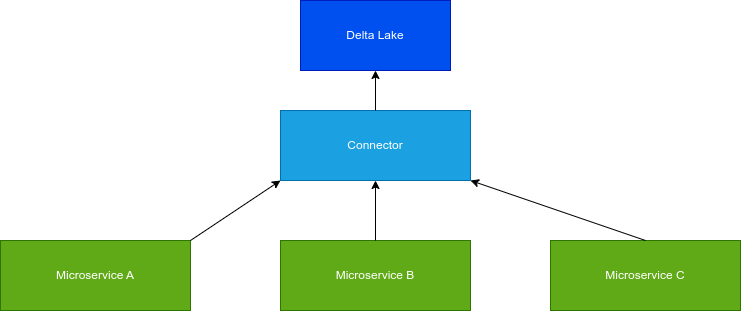
\includegraphics[width=\linewidth]{images/delta-lake-microservices.png}
\caption{Delta lake connectés à des microservices}\label{fig:schema-delta}
\end{figure}

\subsection{Partie Frontend}
Pour la mise en œuvre des microfrontends, Nous avons choisie d'utiliser principalement React pour les microfrontends, l'équipe de développement peut bénéficier de l'écosystème riche et mature de React, ainsi que de sa popularité croissante dans l'industrie du développement frontend. Cependant, il est également mentionné qu'Angular peut être utilisé ultérieurement si nécessaire, offrant ainsi une flexibilité supplémentaire dans le choix des technologies.

\begin{figure}[H]
\centering
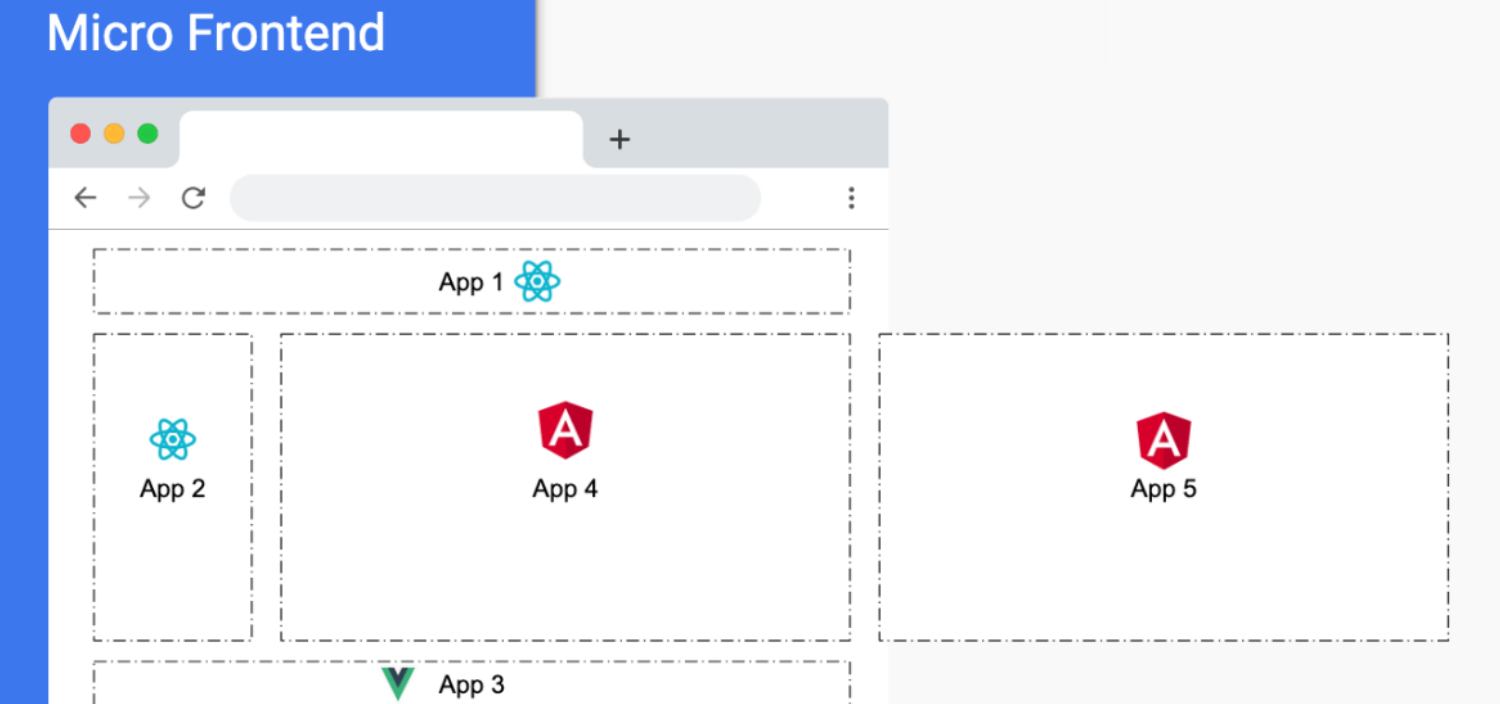
\includegraphics[width=\linewidth]{images/microfrontends.png}
\caption{Schéma des microfrontends}\label{fig:schema-microfrontends}
\end{figure}

\section*{Conclusion}
\addcontentsline{toc}{section}{Conclusion}
Lors de l'évaluation des différentes architectures de données pour Izicap, il est important de comprendre les besoins spécifiques liés à la gestion des fichiers bancaires, des reçus de transactions et des opérations d'agrégation.

Un data warehouse aurait pu être une option envisageable, offrant des structures de données organisées et optimisées pour les requêtes analytiques. Cependant, le principal inconvénient d'un data warehouse réside dans sa nature statique, qui nécessite une modélisation préalable des données et une transformation rigide avant leur chargement. Cela peut poser des défis lors de l'intégration de nouveaux types de fichiers ou de l'évolution des besoins en matière d'agrégation.

D'autre part, un data lake présente des avantages en termes de stockage économique et de flexibilité pour intégrer des données brutes et non structurées. Cependant, il peut être plus complexe de maintenir la qualité des données et la gouvernance, et des compétences techniques spécifiques sont nécessaires pour exploiter efficacement les données du data lake.

Donc, Delta Lake a été privilégié en raison de sa capacité à répondre aux besoins spécifiques d'Izicap en matière de gestion des fichiers bancaires, des reçus de transactions et des opérations d'agrégation. Il offre la flexibilité et la performance nécessaires tout en maintenant l'intégrité des données, ce qui en fait un choix solide pour l'architecture de données de l'entreprise.

En adoptant une approche basée sur les microservices, Izicap peut améliorer la flexibilité, la scalabilité et la maintenance de son application frontend. Cela permettra à l'entreprise de mieux répondre aux besoins changeants de ses utilisateurs, de faciliter la collaboration entre les équipes de développement et d'adopter des technologies innovantes pour offrir une expérience utilisateur optimale.

Les microfrontends offrent plusieurs avantages pour Izicap. Tout d'abord, la modularité inhérente aux microfrontends permet de développer, déployer et maintenir différentes parties de l'interface utilisateur de manière indépendante. Cela favorise la collaboration entre les équipes de développement et permet d'évoluer rapidement et efficacement. Chaque micro-application peut être développée en utilisant le framework et les technologies les plus adaptés à ses besoins spécifiques, ce qui offre une flexibilité technologique essentielle pour Izicap.

En revanche, l'approche monolithique présente des limitations en termes de scalabilité et de flexibilité technologique. Les modifications apportées à une partie de l'application peuvent avoir un impact sur l'ensemble du système, ce qui rend les évolutions plus complexes et risquées. De plus, l'introduction de nouvelles technologies ou frameworks peut être difficile dans une architecture monolithique, ce qui limite les possibilités d'innovation et de modernisation.



    \chapter{Technologies Utilisées}\label{chap:3}
    \addcontentsline{toc}{section}{Introduction}

\section*{Introduction}
Dans ce chapitre, nous examinerons en détail les technologies clés qui sont utilisées dans notre solution pour fournir des fonctionnalités avancées et répondre aux besoins spécifiques de notre projet. Les trois principales technologies que nous aborderons sont Delta Lake, Trino et les Microfrontends.

\section{Delta Lake}

Delta Lake est une technologie de gestion des données qui permet de stocker, gérer et analyser des volumes massifs de données de manière efficace et fiable. Il repose sur une architecture basée sur des fichiers parquet et offre des fonctionnalités avancées telles que la gestion des transactions ACID (Atomicité, Cohérence, Isolation, Durabilité) et la compatibilité avec des outils d'analyse populaires. Delta Lake garantit également l'intégrité des données, la cohérence des requêtes et la prise en charge de la réplication et de la récupération en cas de défaillance.

Le concept de `lakehouse' est rendu possible grâce à Delta Lake. Il s'agit d'une architecture de données qui combine les avantages des entrepôts de données et des lacs de données, en offrant une approche unique et cohérente pour la gestion des données. Les données sont stockées au format Parquet dans le lac de données, permettant ainsi un traitement continu et par lots.
\begin{itemize}
    \item \textbf{Permet une architecture  Lakehouse:} Delta Lake permet une architecture de données continue et simplifiée qui permet aux organisations de gérer et de traiter d'énormes volumes de données en continu et par lots sans les tracas de gestion et d'exploitation liés à la gestion séparée du streaming, des data warehouses et des lacs de données.
    \item \textbf{Permet une gestion intelligente des données pour les lacs de données:} Delta Lake offre une gestion efficace et évolutive des métadonnées, qui fournit des informations sur les volumes de données massifs dans les lacs de données. Grâce à ces informations, les tâches de gouvernance et de gestion des données se déroulent plus efficacement.
    \item \textbf{Application du schéma pour une meilleure qualité des données:} Étant donné que les lacs de données n'ont pas de schéma défini, il devient facile pour les données mauvaises/incompatibles d'entrer dans les systèmes de données. La qualité des données est améliorée grâce à la validation automatique du schéma, qui valide la compatibilité DataFrame et table avant les écritures.
    \item \textbf{Permet la transaction ACID:} La plupart des architectures de données organisationnelles impliquent de nombreux mouvements ETL et ELT entrant et sortant du stockage de données, ce qui l'ouvre à plus de complexité et d'échecs aux points d'entrée des nœuds. Delta Lake garantit la durabilité et la persistance des données pendant l'ETL et d'autres opérations de données. Delta Lake capture toutes les modifications apportées aux données pendant les opérations de données dans un journal des transactions, garantissant ainsi l'intégrité et la fiabilité des données pendant les opérations de données.
\end{itemize}

\section{Principaux avantages et caractéristiques de Delta Lake}
\begin{flushleft}
	Avec Delta Lake, les données sont stockées dans un format optimisé, tel que Parquet, dans un lac de données. Ce format facilite le traitement efficace des requêtes, quel que soit le mode d'accès aux données, qu'il s'agisse d'un traitement streaming ou par batch.
\end{flushleft}

\begin{figure}[H]
\centering
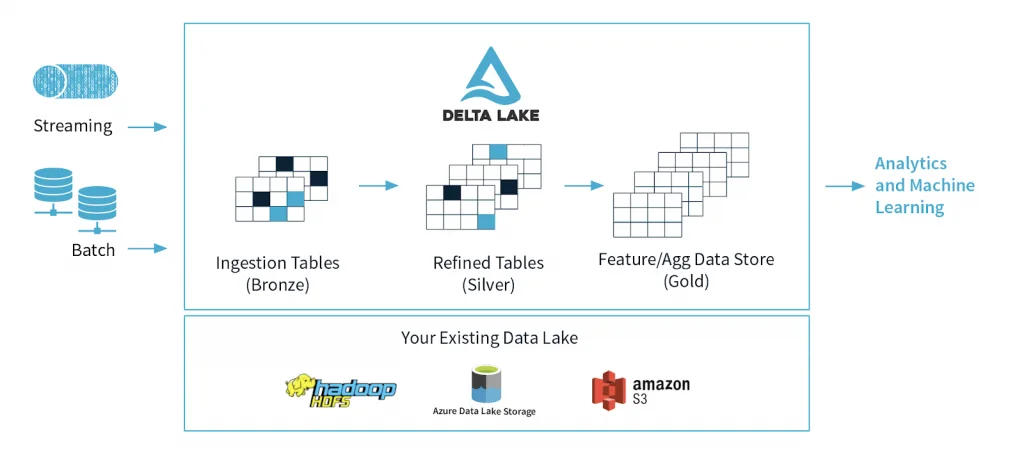
\includegraphics[width=\linewidth]{images/delta_lake_architecture.png}
\caption{Architecture multi-sauts de Delta Lake}\label{fig:delta-lake-architecture}
\end{figure}

\begin{itemize}
	\item[\textbullet] \textbf{Pistes d'audit et historique:}Dans Delta Lake, chaque écriture existe en tant que transaction et est enregistrée en série dans un journal des transactions. Par conséquent, toutes les modifications ou validations apportées au journal des transactions sont enregistrées, laissant une trace complète à utiliser dans les audits historiques, la gestion des versions ou à des fins de voyage dans le temps. Cette fonctionnalité de Delta Lake permet de garantir l'intégrité et la fiabilité des données pour les opérations de données d'entreprise.
	\item[\textbullet] \textbf{Voyager dans le temps et versionner les données:} Étant donné que chaque écriture crée une nouvelle version et stocke l'ancienne version dans le journal des transactions, les utilisateurs peuvent afficher/restaurer les anciennes versions de données en fournissant l'horodatage ou le numéro de version d'une table ou d'un répertoire existant à l'API de lecture Sparks\@. À l'aide du numéro de version fourni, Delta Lake construit ensuite un instantané complet de la version avec les informations fournies par le journal des transactions. Les retours en arrière et la gestion des versions jouent un rôle essentiel dans l'expérimentation de l'apprentissage automatique, où les scientifiques des données modifient de manière itérative les hyperparamètres pour former des modèles et peuvent revenir aux modifications si nécessaire.
	\item[\textbullet] \textbf{Unifie le traitement par lots et par flux:} Chaque table d'un Delta Lake est un puits de lot et de flux. Avec le streaming structuré Sparks, les organisations peuvent diffuser et traiter efficacement les données de streaming. De plus, grâce à la gestion efficace des métadonnées, à la facilité d'évolutivité et à la qualité ACID de chaque transaction, l'analyse en temps quasi réel devient possible sans utiliser une architecture de données à deux niveaux plus compliquée.
	\item[\textbullet] \textbf{Gestion efficace et évolutive des métadonnées:} Delta Lakes stocke les informations de métadonnées dans le journal des transactions et exploite la puissance de traitement distribuée de Spark pour traiter rapidement, lire et gérer efficacement de gros volumes de métadonnées de données, améliorant ainsi la gouvernance des données.
	\item[\textbullet] \textbf{transactions ACID:} Delta Lakes garantit que les utilisateurs voient toujours une vue de données cohérente dans une table ou un répertoire. Il garantit cela en capturant chaque modification effectuée dans un journal de transactions et en l'isolant au niveau d'isolation le plus fort, le niveau sérialisable. Au niveau sérialisable, chaque opération existante a et suit une séquence en série qui, lorsqu'elle est exécutée une par une, fournit le même résultat que celui indiqué dans le tableau.
	\item[\textbullet] \textbf{Opérations du langage de manipulation de données:} Delta Lakes prend en charge les opérations DML telles que les mises à jour, les suppressions et les fusions, qui jouent un rôle dans les opérations de données complexes telles que la capture de données de modification (CDC), les upserts en continu et la dimension à évolution lente (SCD). Des opérations comme CDC assurent la synchronisation des données dans tous les systèmes de données et minimisent le temps et les ressources consacrés aux opérations ELT. Par exemple, en utilisant le CDC, au lieu d'ETL toutes les données disponibles, seules les données récemment mises à jour depuis la dernière opération subissent une transformation.
	\item[\textbullet] \textbf{Schema Enforcement:} Delta Lakes effectue une validation automatique du schéma en vérifiant un ensemble de règles pour déterminer la compatibilité d'une écriture d'un DataFrame vers une table. L'une de ces règles est l'existence de toutes les colonnes DataFrame dans la table cible. Une occurrence d'une colonne supplémentaire ou manquante dans le DataFrame génère une erreur d'exception. Une autre règle est que le DataFrame et la table cible doivent contenir les mêmes types de colonnes, ce qui, sinon, déclenchera une exception. Delta Lake utilise également DDL (Data Definition Language) pour ajouter explicitement de nouvelles colonnes. Cette fonctionnalité de lac de données permet d'éviter l'ingestion de données incorrectes, garantissant ainsi une qualité élevée des données.
	\item[\textbullet] \textbf{Compatibilité avec l'API de Spark:} Delta Lake est basé sur Apache Spark et est entièrement compatible avec l'API Spark, qui permet de créer des pipelines de données volumineuses efficaces et fiables.
	\item[\textbullet] \textbf{Flexibilité et intégration:} Delta Lake est une couche de stockage open source et utilise le format Parquet pour stocker des fichiers de données, ce qui favorise le partage de données et facilite l'intégration avec d'autres technologies et stimule l'innovation.
\end{itemize}

\section{Trino}

Trino, anciennement connu sous le nom de Presto, est un moteur de requêtes SQL distribué et open-source. Il est conçu pour exécuter des requêtes interactives et analytiques à grande échelle sur des données hétérogènes et distribuées. Trino offre une grande polyvalence en permettant l'accès à différents types de sources de données, qu'il s'agisse de bases de données relationnelles, de systèmes de fichiers, de sources de données en temps réel ou de services de stockage cloud. Grâce à sa conception distribuée, Trino permet des performances élevées et une scalabilité horizontale, ce qui en fait un outil essentiel pour l'analyse des données dans notre solution.

\begin{figure}[H]
\centering
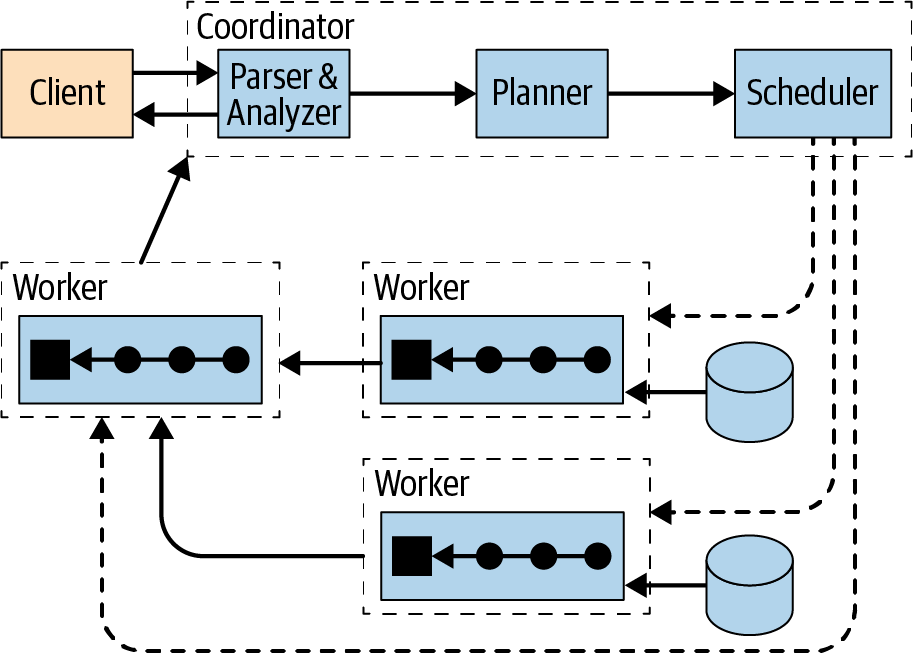
\includegraphics[width=0.8\linewidth]{images/trino_architecture.png}
\caption{Vue d'ensemble de l'architecture Trino avec le coordinateur et les workers}\label{fig:trino-architecture}
\end{figure}

\begin{enumerate}
	\item Un coordinateur est un serveur Trino qui gère les requêtes entrantes et gère les workers pour exécuter les requêtes.
	\item Un worker est un serveur Trino responsable de l'exécution des tâches et du traitement des données.
	\item Le service de découverte s'exécute généralement sur le coordinateur et permet aux workers de s'inscrire pour participer au cluster.
	\item Toutes les communications et tous les transferts de données entre les clients, le coordinateur et les workers utilisent des interactions basées sur REST sur HTTP/HTTPS.
\end{enumerate}

\section{Springboot}

Spring Boot est un framework open-source pour le développement d'applications Java. Il fournit une approche simplifiée et conventionnelle pour créer des applications Java autonomes, prêtes à être déployées, sans nécessiter une configuration complexe.

L'un des principaux avantages de Spring Boot est sa capacité à réduire la configuration boilerplate et à simplifier le développement d'applications en fournissant des définitions de configuration par défaut intelligentes et en automatisant de nombreux aspects du développement. Il intègre également un serveur d'applications embarqué, ce qui facilite le déploiement et l'exécution de l'application sans avoir besoin d'un serveur d'applications externe.

Spring Boot suit le paradigme de la programmation orientée annotation, où les annotations sont utilisées pour configurer et orchestrer les différentes parties de l'application. Il offre une large gamme de fonctionnalités, telles que l'injection de dépendances, la configuration externe, la gestion des erreurs, la sécurité, l'accès aux données, etc. Ces fonctionnalités sont regroupées dans des starters, qui sont des dépendances prédéfinies facilitant l'ajout de fonctionnalités spécifiques à l'application.

Grâce à son approche simplifiée, Spring Boot permet aux développeurs de se concentrer davantage sur la logique métier de leur application plutôt que sur des tâches de configuration fastidieuses. Il favorise également les bonnes pratiques de développement, telles que la séparation des préoccupations et la modularité, ce qui rend les applications plus maintenables et évolutives.


\section{Keycloak}

Keycloak est une solution open-source de gestion des identités et des accès (Identity and Access Management) développée par Red Hat. Il fournit des fonctionnalités complètes pour la gestion des utilisateurs, l'authentification, l'autorisation et la sécurisation des applications.

Keycloak permet de centraliser et de simplifier la gestion des identités au sein d'une infrastructure informatique. Il offre des fonctionnalités telles que l'inscription des utilisateurs, l'authentification à plusieurs facteurs, la gestion des rôles et des autorisations, la gestion des sessions, ainsi que l'intégration avec des protocoles d'authentification et d'autorisation courants tels que OAuth 2.0 et OpenID Connect.

Keycloak offre un ensemble de fonctionnalités pour gérer les rôles, les administrateurs, les utilisateurs et les mots de passe. Voici comment Keycloak aborde ces aspects:

\begin{enumerate}
	\item Keycloak permet de définir des rôles au niveau du royaume (realm) ou au niveau de l'application. Les rôles peuvent être créés et attribués aux utilisateurs pour définir leurs autorisations et leurs accès.
	\item Les administrateurs Keycloak peuvent créer, gérer et assigner des rôles aux utilisateurs via l'interface d'administration ou via l'API de gestion.
	\item Les rôles peuvent être utilisés pour contrôler l'accès aux fonctionnalités, aux pages et aux ressources au sein de l'application.
	\item Keycloak propose des rôles d'administration spécifiques tels que "admin" ou "superadmin" qui permettent aux utilisateurs d'effectuer des tâches d'administration, telles que la gestion des clients, des utilisateurs, des rôles, etc.
	\item Les utilisateurs peuvent se connecter à l'aide de leurs identifiants (nom d'utilisateur et mot de passe) ou d'autres méthodes d'authentification prises en charge, telles que l'authentification à deux facteurs, OAuth 2.0, etc.
	\item Keycloak prend en charge l'authentification basée sur les utilisateurs et fournit une interface d'inscription pour permettre aux utilisateurs de créer leurs comptes.
	\item Keycloak offre également des fonctionnalités d'authentification avancées, telles que l'authentification à deux facteurs, l'authentification sociale (via des fournisseurs d'identité tels que Google, Facebook, etc.) et l'authentification basée sur des certificats.
\end{enumerate}

\section{Kafka}

Kafka est une plateforme de streaming de données distribuée et évolutive, conçue pour gérer efficacement la transmission et le traitement de flux de données en temps réel. Elle a été développée par Apache Software Foundation.

Kafka est basé sur une architecture de journal de messages distribué, où les données sont stockées sous forme de flux de messages dans des "topics". Les producteurs de données envoient des messages à des "topics" spécifiques, tandis que les consommateurs s'abonnent à ces "topics" pour récupérer les messages. Cela permet une communication asynchrone et une séparation claire entre les producteurs et les consommateurs de données.

Les principales caractéristiques de Kafka incluent:

\begin{enumerate}
	\item Scalabilité: Kafka est conçu pour gérer de gros volumes de données et peut être mis à l'échelle horizontalement pour répondre aux besoins de performance croissants. Il peut gérer des charges de travail élevées et traiter des milliers de messages par seconde.
	\item Tolérance aux pannes: Kafka garantit une haute disponibilité et une tolérance aux pannes en répliquant les données sur plusieurs nœuds du cluster. Cela garantit la fiabilité et la disponibilité des données, même en cas de défaillance d'un ou plusieurs nœuds.
	\item Durabilité des données: Les messages stockés dans Kafka sont persistants et peuvent être conservés pendant une période définie. Cela permet de rejouer les messages et de récupérer les données en cas de besoin, ce qui est essentiel pour les cas d'utilisation nécessitant une conservation à long terme des données.
	\item Traitement de flux: Kafka est conçu pour le traitement de flux en temps réel. Il permet aux applications de consommer des flux de données en continu et de les traiter en temps réel, ce qui est crucial pour les cas d'utilisation nécessitant une analyse en temps réel, des pipelines de données, etc.
	\item Intégration avec d'autres outils: Kafka s'intègre facilement avec d'autres outils et frameworks tels que Spark, Hadoop, Flink, etc. Cela permet une intégration transparente avec l'écosystème Big Data et facilite l'ingestion, le traitement et la diffusion des données.
\end{enumerate}

\begin{figure}[H]
\centering
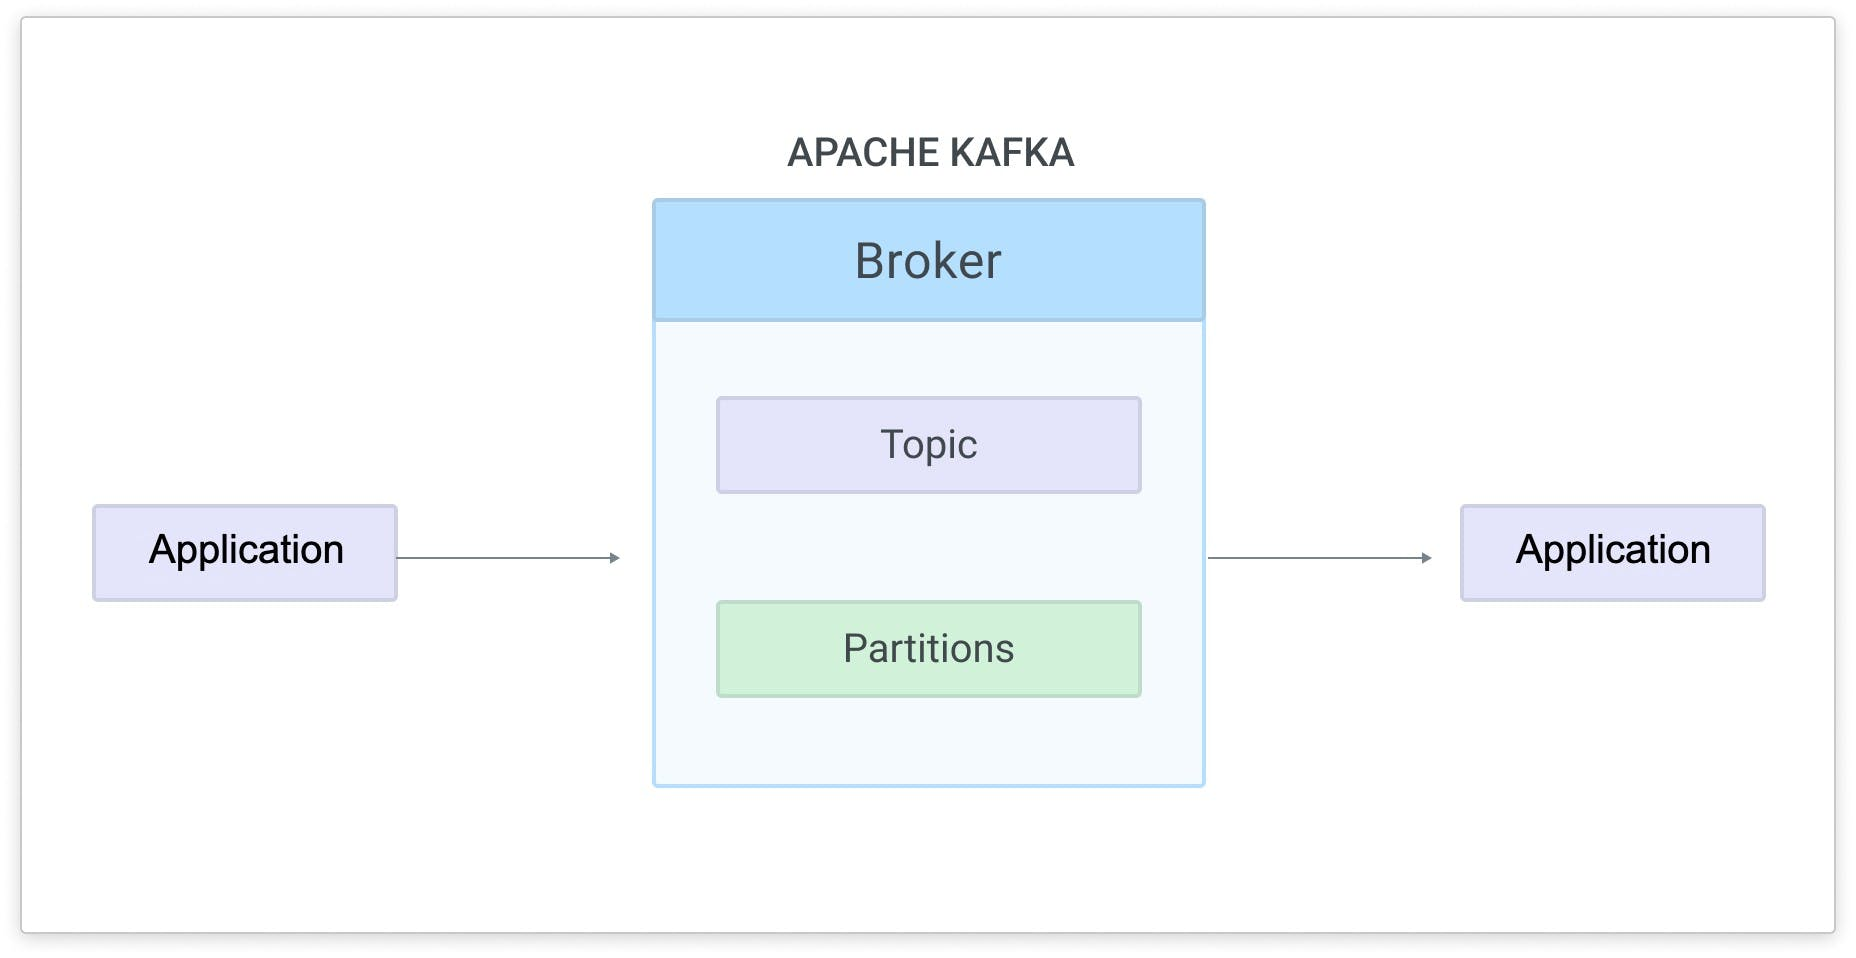
\includegraphics[width=\linewidth]{images/kafka.jpg}
\caption{Architecture Kafka}\label{fig:kafka}
\end{figure}


    \chapter{Implementation de la solution}\label{chap:4}
    \addcontentsline{toc}{section}{Introduction}

\section*{Introduction}

Ce chapitre se concentre sur l'implémentation de la solution, en mettant l'accent sur le choix du connecteur pour manipuler Delta Lake. Nous discuterons de l'étude de faisabilité des différents connecteurs et de leur impact sur la modularité, les performances et la sécurité.

\section{Étude de faisabilité}
Lors de notre étude de faisabilité, nous avons examiné plusieurs options de connecteurs pour manipuler Delta Lake. Voici un aperçu des connecteurs que nous avons explorés:

\begin{enumerate}
    \item \textbf{Delta Standalone:} Nous avons tenté d'utiliser Delta Standalone, qui est un connecteur indépendant de Spark. Cependant, nous avons constaté que Delta Standalone ne prend en charge que des snapshots de timestamp et ne permet pas les requêtes. De plus, il peut parfois être lourd lors de la récupération de plusieurs enregistrements, ce qui affecte les performances.
    \item \textbf{Delta Sharing Server:} Delta Sharing Server est une autre option qui nécessite son propre serveur. Bien qu'il soit populaire avec Rust et Python, nous avons constaté que l'utilisation de Delta Sharing Server avec Java ne fournit pas toutes les options disponibles et manque de documentation détaillée.
    \item \textbf{Spark:} Spark est une option faisable et déjà disponible pour manipuler Delta Lake. Cependant, il nécessite une version spécifique de Spring Boot (2.7-) avec une configuration Maven très spécifique. Bien que Spark offre de nombreuses fonctionnalités et soit bien intégré à l'écosystème de Big Data, son utilisation peut être complexe et nécessite une configuration précise.
    \item \textbf{Trino:} Trino est un autre connecteur que nous avons exploré. Cependant, il nécessite son propre serveur et une base de données relationnelle (Hive). Trino offre plusieurs avantages, notamment la possibilité d'utiliser du SQL standard et un connecteur Java JDBC pour accéder à Delta Lake. Cela offre une flexibilité et une facilité d'utilisation accrues.
\end{enumerate}

\section{Benchmark entre Trino et Spark}
Trino est un moteur de requêtage distribué et rapide conçu pour exécuter des requêtes SQL interactives sur de grands ensembles de données. Spark, d'autre part, est un système de traitement distribué populaire qui prend également en charge le requêtage de données à grande échelle.
Pour cette étude de benchmark, nous allons évaluer les performances de Trino et Spark sur le requêtage de données stockées dans Delta Lake (S3 Amazon dans notre cas), un format de stockage de données optimisé pour les analyses analytiques.

\subsection{Architecture}
Les deux schémas suivant représentent l’architecture respective des deux POC (Proof Of Concept) SPARK et TRINO.

\begin{figure}[H]
\centering
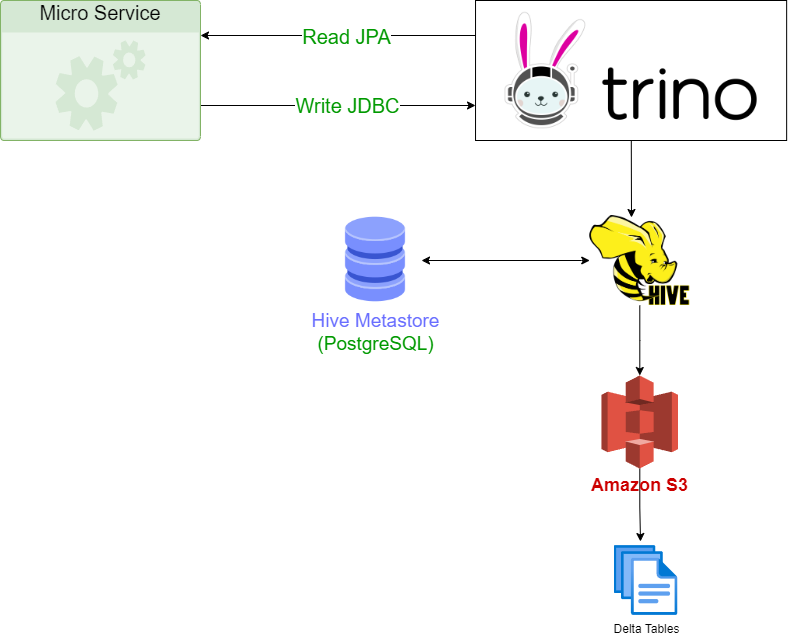
\includegraphics[width=\linewidth]{images/trino_microservice.png}
\caption{Architecture TRINO}\label{fig:arch-trino}
\end{figure}

\begin{figure}[H]
\centering
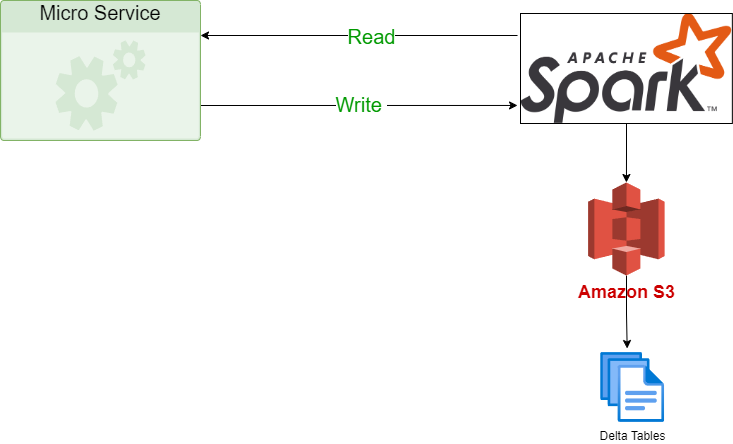
\includegraphics[width=\linewidth]{images/archi-spark.png}
\caption{Architecture SPARK}\label{fig:arch-spark}
\end{figure}
    
\subsection{Temps d'exécution}
\begin{enumerate}
    \item[$\bullet$] \textbf{Trino:} Trino est connu pour sa vitesse d'exécution élevée. Il utilise une architecture optimisée pour exécuter des requêtes SQL de manière très rapide, en exploitant la parallélisation et l'optimisation des requêtes. Trino peut fournir des temps d'exécution courts en ce qui concerne les requêtes sur Delta Lake.
    \item[$\bullet$] \textbf{Spark:} Spark est également conçu pour offrir des performances élevées, mais il peut nécessiter plus de temps pour lire les données à partir du disque. Cependant, Spark peut offrir des performances élevées lorsqu'il est utilisé avec des opérations de transformation complexes, grâce à son modèle de calcul distribué basé sur le disque.
\end{enumerate}

Nous avons effectué un test de performance sur une table Delta de 2 giga-octets en utilisant 2 ordinateurs:
\begin{enumerate}
    \item Le premier PC «DELL Latitude 5530» ou nous allons lancer les images Docker suivantes:
    \item \begin{enumerate}
        \item[$\bullet$] \textbf{Trino:} c’est l’image du serveur Trino pour l'interrogation de données distribué avec le langage SQL 
        \item[$\bullet$] \textbf{Hive:} Il sera utilisé conjointement avec Trino afin d’interroger et analyser des données stockées dans Hive grâce à la compatibilité entre les deux systèmes et le partage des métadonnées via le Hive Metastore.
        \item[$\bullet$] \textbf{PostgreSQL:} Il sera utilisé afin de stocker les métadonnées des tables Delta, des schémas et des partitions, facilitant ainsi la gestion, la découverte et l'accès aux données dans un environnement distribué. Il offre également des fonctionnalités d'optimisation des requêtes et de gestion des autorisations pour améliorer les performances et la sécurité des analyses de données.
        \item[$\bullet$] \textbf{AWS:} Où les delta tables sont trouvés.
    \end{enumerate}
    \item Le Dexième PC «ASUS ROG G752 VT» c’est là ou sera exécuté les micro-services springboot de SPARK et de TRINO.\@
\end{enumerate}

La configuration utilisée lors des tests est la suivante:
\begin{table}[h]
\centering
\label{tab:caracteristiques}
\begin{tabular}{|l|l|}
\hline
\textbf{Composant} & \textbf{Spécifications} \\ \hline
Processeur & 12th Gen Intel\textsuperscript{®} Core\textsuperscript{TM} i7-1255U 1.70 - 4.8 GHz \\ \hline
Fréquence processeur & 2.6 - 3.2 GHz \\ \hline
Mémoire vive & 24 GO \\ \hline
Type de mémoire vive & DDR4 \\ \hline
Puce graphique & Intel Iris Xe Graphics \\ \hline
Disque dur & 512GB PCIe NVMe Class 35 SSD \\ \hline
Type du système d'exploitation & Windows 11 64 bits \\ \hline
\end{tabular}
\caption{Caractéristiques techniques du PC « DEL Latitude 5530 »}
\end{table}

\begin{table}[h]
\centering
\label{tab:caracteristiques-2}
\begin{tabular}{|l|l|}
\hline
\textbf{Composant} & \textbf{Spécifications} \\ \hline
Processeur & Intel Core i7-6700HQ \\ \hline
Fréquence processeur & 2.6 - 3.2 GHz \\ \hline
Mémoire vive & 24 GO DDR4 \\ \hline
Disque dur & 1TO SSD + 1TO HDD \\ \hline
Type de mémoire vive & DDR4-SDRAM \\ \hline
Puce graphique & Nvidia GeForce GTX 970M \\ \hline
Quantité de mémoire graphique & 3072 Mo dédiée \\\hline
Type du système d'exploitation & Windows 10 64 bits \\ \hline
\end{tabular}
\caption{Caractéristiques techniques du PC «ASUS ROG G752 VT»}
\end{table}

Les résultats sont les suivants:

\begin{table}[h]
\centering
\label{tab:resultats}
\begin{tabular}{|l|l|l|}
\hline
\multirow{2}{*}{\textbf{Requêtes}} & \multicolumn{2}{c|}{\textbf{Implémentation}} \\ \cline{2-3}
& \textbf{Spark (s)} & \textbf{Trino (s)} \\ \hline
SELECT (par page et par limite de résultats par page - 100 par page) & 1.2 & 0.43 \\ \hline
Agrégation et regroupement & 2.1 & 0.8 \\ \hline
Tri & 2.2 & 0.8 \\ \hline
\end{tabular}
\caption{Caractéristiques techniques du PC «ASUS ROG G752 VT»}
\end{table}

\subsection{Gestion de la mémoire}
\begin{enumerate}
    \item[$\bullet$] \textbf{Trino:} Trino utilise principalement la mémoire pour accélérer le traitement des requêtes. Il dispose d'un moteur de requêtage en mémoire qui optimise l'accès aux données et minimise les temps d'accès. Cependant, cela signifie que Trino peut nécessiter une quantité de mémoire significative pour traiter de grands ensembles de données.
    \item[$\bullet$] \textbf{Spark:} Spark utilise un modèle de calcul distribué basé sur le disque, ce qui signifie que les données sont généralement stockées sur le disque et chargées en mémoire selon les besoins. Cela permet à Spark de gérer des ensembles de données beaucoup plus volumineux que ce qui peut tenir en mémoire.
\end{enumerate}
    
\subsection{Écosystème et intégrations}
\begin{enumerate}
    \item[$\bullet$] \textbf{Trino:} Trino dispose d'un écosystème en pleine croissance avec une large gamme de connecteurs et d'intégrations, ce qui permet d'accéder à différentes sources de données, y compris Delta Lake. Il est compatible avec divers outils de visualisation et de traitement des données.
    \item[$\bullet$] \textbf{Spark:} Spark est un projet mature avec un écosystème riche d'outils, de bibliothèques et de connecteurs. Il bénéficie d'une large communauté de développeurs et de nombreuses ressources d'apprentissage. Spark prend également en charge le traitement de données en continu et le traitement par lots.
\end{enumerate}

\subsection{Évolutivité}
\begin{enumerate}
    \item[$\bullet$] \textbf{Trino:} Trino est conçu pour être hautement évolutif et peut gérer de grands ensembles de données. Il peut être facilement configuré pour s'adapter à des charges de travail intensives et à des volumes de données importants.
    \item[$\bullet$] \textbf{Spark:} Spark est également conçu pour l'évolutivité et peut traiter des ensembles de données massifs. Il dispose d'un système de traitement distribué qui peut s'adapter à différentes configurations de clusters et de ressources.
\end{enumerate}

\subsection{Support des fonctionnalités Delta Lake}
\begin{enumerate}
    \item[$\bullet$] \textbf{Trino:} Trino dispose d'un connecteur officiel pour Delta Lake, ce qui lui permet de lire et d'écrire des données dans Delta Lake. Il prend en charge les fonctionnalités essentielles de Delta Lake, telles que la gestion des transactions ACID, les mises à jour incrémentielles et les opérations de fusion ("merge").
    \item[$\bullet$] \textbf{Spark:} Spark dispose également d'un support intégré pour Delta Lake. Il offre des fonctionnalités avancées de gestion des données Delta, notamment la prise en charge des transactions ACID, des opérations de fusion performantes et des mécanismes de contrôle de version des données.
\end{enumerate}

\subsection{Facilité d'utilisation}
\begin{enumerate}
    \item[$\bullet$] \textbf{Trino:} Trino offre une interface SQL standard, ce qui facilite son utilisation pour les utilisateurs familiers avec SQL. Il propose également des outils de requêtage interactif conviviaux et des options de configuration flexibles.
    \item[$\bullet$] \textbf{Spark:} Spark propose une interface SQL via Spark SQL, mais il est également orienté vers le traitement de données par le biais d'un API plus large. Spark peut être plus complexe à utiliser pour les utilisateurs moins familiers avec les concepts du traitement distribué.
\end{enumerate}

\subsection{Autres statistiques}

\begin{longtable}{|p{0.23\linewidth}|p{0.35\linewidth}|p{0.42\linewidth}|}
\hline
\textbf{} & \textbf{Spark} & \textbf{Trino} \\ \hline
\textbf{Expérience \newline Développeur} & 

\includegraphics[width=0.28in,height=0.28in]{images/image3.png}
\includegraphics[width=0.28in,height=0.28in]{images/image3.png}\newline
La syntaxe de Spark exige que les PME aient une expérience en ingénierie de données &

\includegraphics[width=0.28in,height=0.28in]{images/image3.png}
\includegraphics[width=0.28in,height=0.28in]{images/image3.png}
\includegraphics[width=0.28in,height=0.28in]{images/image3.png}\newline
Une interface SQL standard, ce qui facilite son utilisation pour les utilisateurs familiers avec SQL \\ \hline
\textbf{Coût} & 
Équipe: 
\includegraphics[width=0.33in,height=0.35in]{images/image4.jpg}
\includegraphics[width=0.33in,height=0.35in]{images/image4.jpg}\newline
Infrastructure: \textcolor[RGB]{0, 128, 0}{\textbf{\large \$}} & 
Équipe: 
\includegraphics[width=0.33in,height=0.35in]{images/image4.jpg}
\includegraphics[width=0.33in,height=0.35in]{images/image4.jpg}\newline
Infrastructure: \textcolor[RGB]{0, 128, 0}{\textbf{\large \$}} \\ \hline
\textbf{Fiabilité} & 

\includegraphics[width=0.28in,height=0.28in]{images/image3.png}
\includegraphics[width=0.28in,height=0.28in]{images/image3.png}
\includegraphics[width=0.28in,height=0.28in]{images/image3.png}\newline
Produit mature maintenu en interne et pris en charge par Google Dataproc &

\includegraphics[width=0.28in,height=0.28in]{images/image3.png}
\includegraphics[width=0.28in,height=0.28in]{images/image3.png}\newline
A été en panne à quelques reprises car l'équipe interne apprend à maintenir et à évoluer \\ \hline
\textbf{Caractéristiques et Open sources} & 

\includegraphics[width=0.28in,height=0.28in]{images/image3.png}
\includegraphics[width=0.28in,height=0.28in]{images/image3.png}
\includegraphics[width=0.28in,height=0.28in]{images/image3.png}\newline
A été soutenu par la communauté open source depuis 2014 &

\includegraphics[width=0.28in,height=0.28in]{images/image3.png}
\includegraphics[width=0.28in,height=0.28in]{images/image3.png}
\includegraphics[width=0.28in,height=0.28in]{images/image3.png}\newline
A été soutenu par la communauté open source depuis 2019. Shopify a apporté des contributions. \\ \hline
\textbf{Usage} & 
\textasciitilde800,000 emplois/jour & 
3000 utilisateurs actifs/semaine \newline
\textasciitilde200,000 requêtes/semaine \\ \hline
\end{longtable}

\section{Schématisation de la Solution}

Dans le cadre de la schématisation de la solution, nous avons opté pour une architecture basée sur des microservices, utilisant les technologies suivantes : Spring Data, JPA, Hibernate, JDBC et Trino.

Les microservices sont développés en utilisant Spring Data, qui fournit une abstraction de haut niveau pour interagir avec la base de données. Cela permet d'utiliser des annotations et des interfaces pour définir les entités, les requêtes et les opérations de persistance. JPA (Java Persistence API) est utilisé comme couche d'interface pour interagir avec la base de données, tandis que Hibernate est utilisé comme fournisseur de persistance, permettant la gestion des objets Java et leur mapping vers Trino.

La communication entre les microservices est assurée par un broker Kafka. Kafka est une plateforme de streaming distribuée qui permet aux microservices d'échanger des messages en temps réel. Les microservices publient des événements sur des sujets Kafka, et d'autres microservices peuvent s'abonner à ces sujets pour recevoir les événements correspondants.

Pour gérer l'authentification et l'autorisation, nous utilisons Spring Cloud Gateway. Ce composant reçoit les appels de services provenant des applications Web, mobiles ou de bureau. Ces applications envoient un jeton JWT (JSON Web Token) à Spring Cloud Gateway pour authentification. Ce dernier vérifie la disponibilité du jeton en contactant Keycloak, qui est responsable de la gestion des identités et des accès. Une fois le jeton validé, Spring Cloud Gateway autorise la demande à passer vers les microservices.

Les microservices communiquent avec Trino en utilisant le connecteur JDBC\@. Trino est responsable de l'interrogation et du traitement des données sur une grande quantité de sources de données. Il stocke les métadonnées dans Hive, qui est un entrepôt de données basé sur Hadoop. Trino utilise également le concept de tables Delta pour gérer les modifications incrémentielles des données. Ces tables Delta sont stockées sur AWS (Amazon Web Services), offrant une solution de stockage évolutive et fiable.

\begin{figure}[H]
\centering
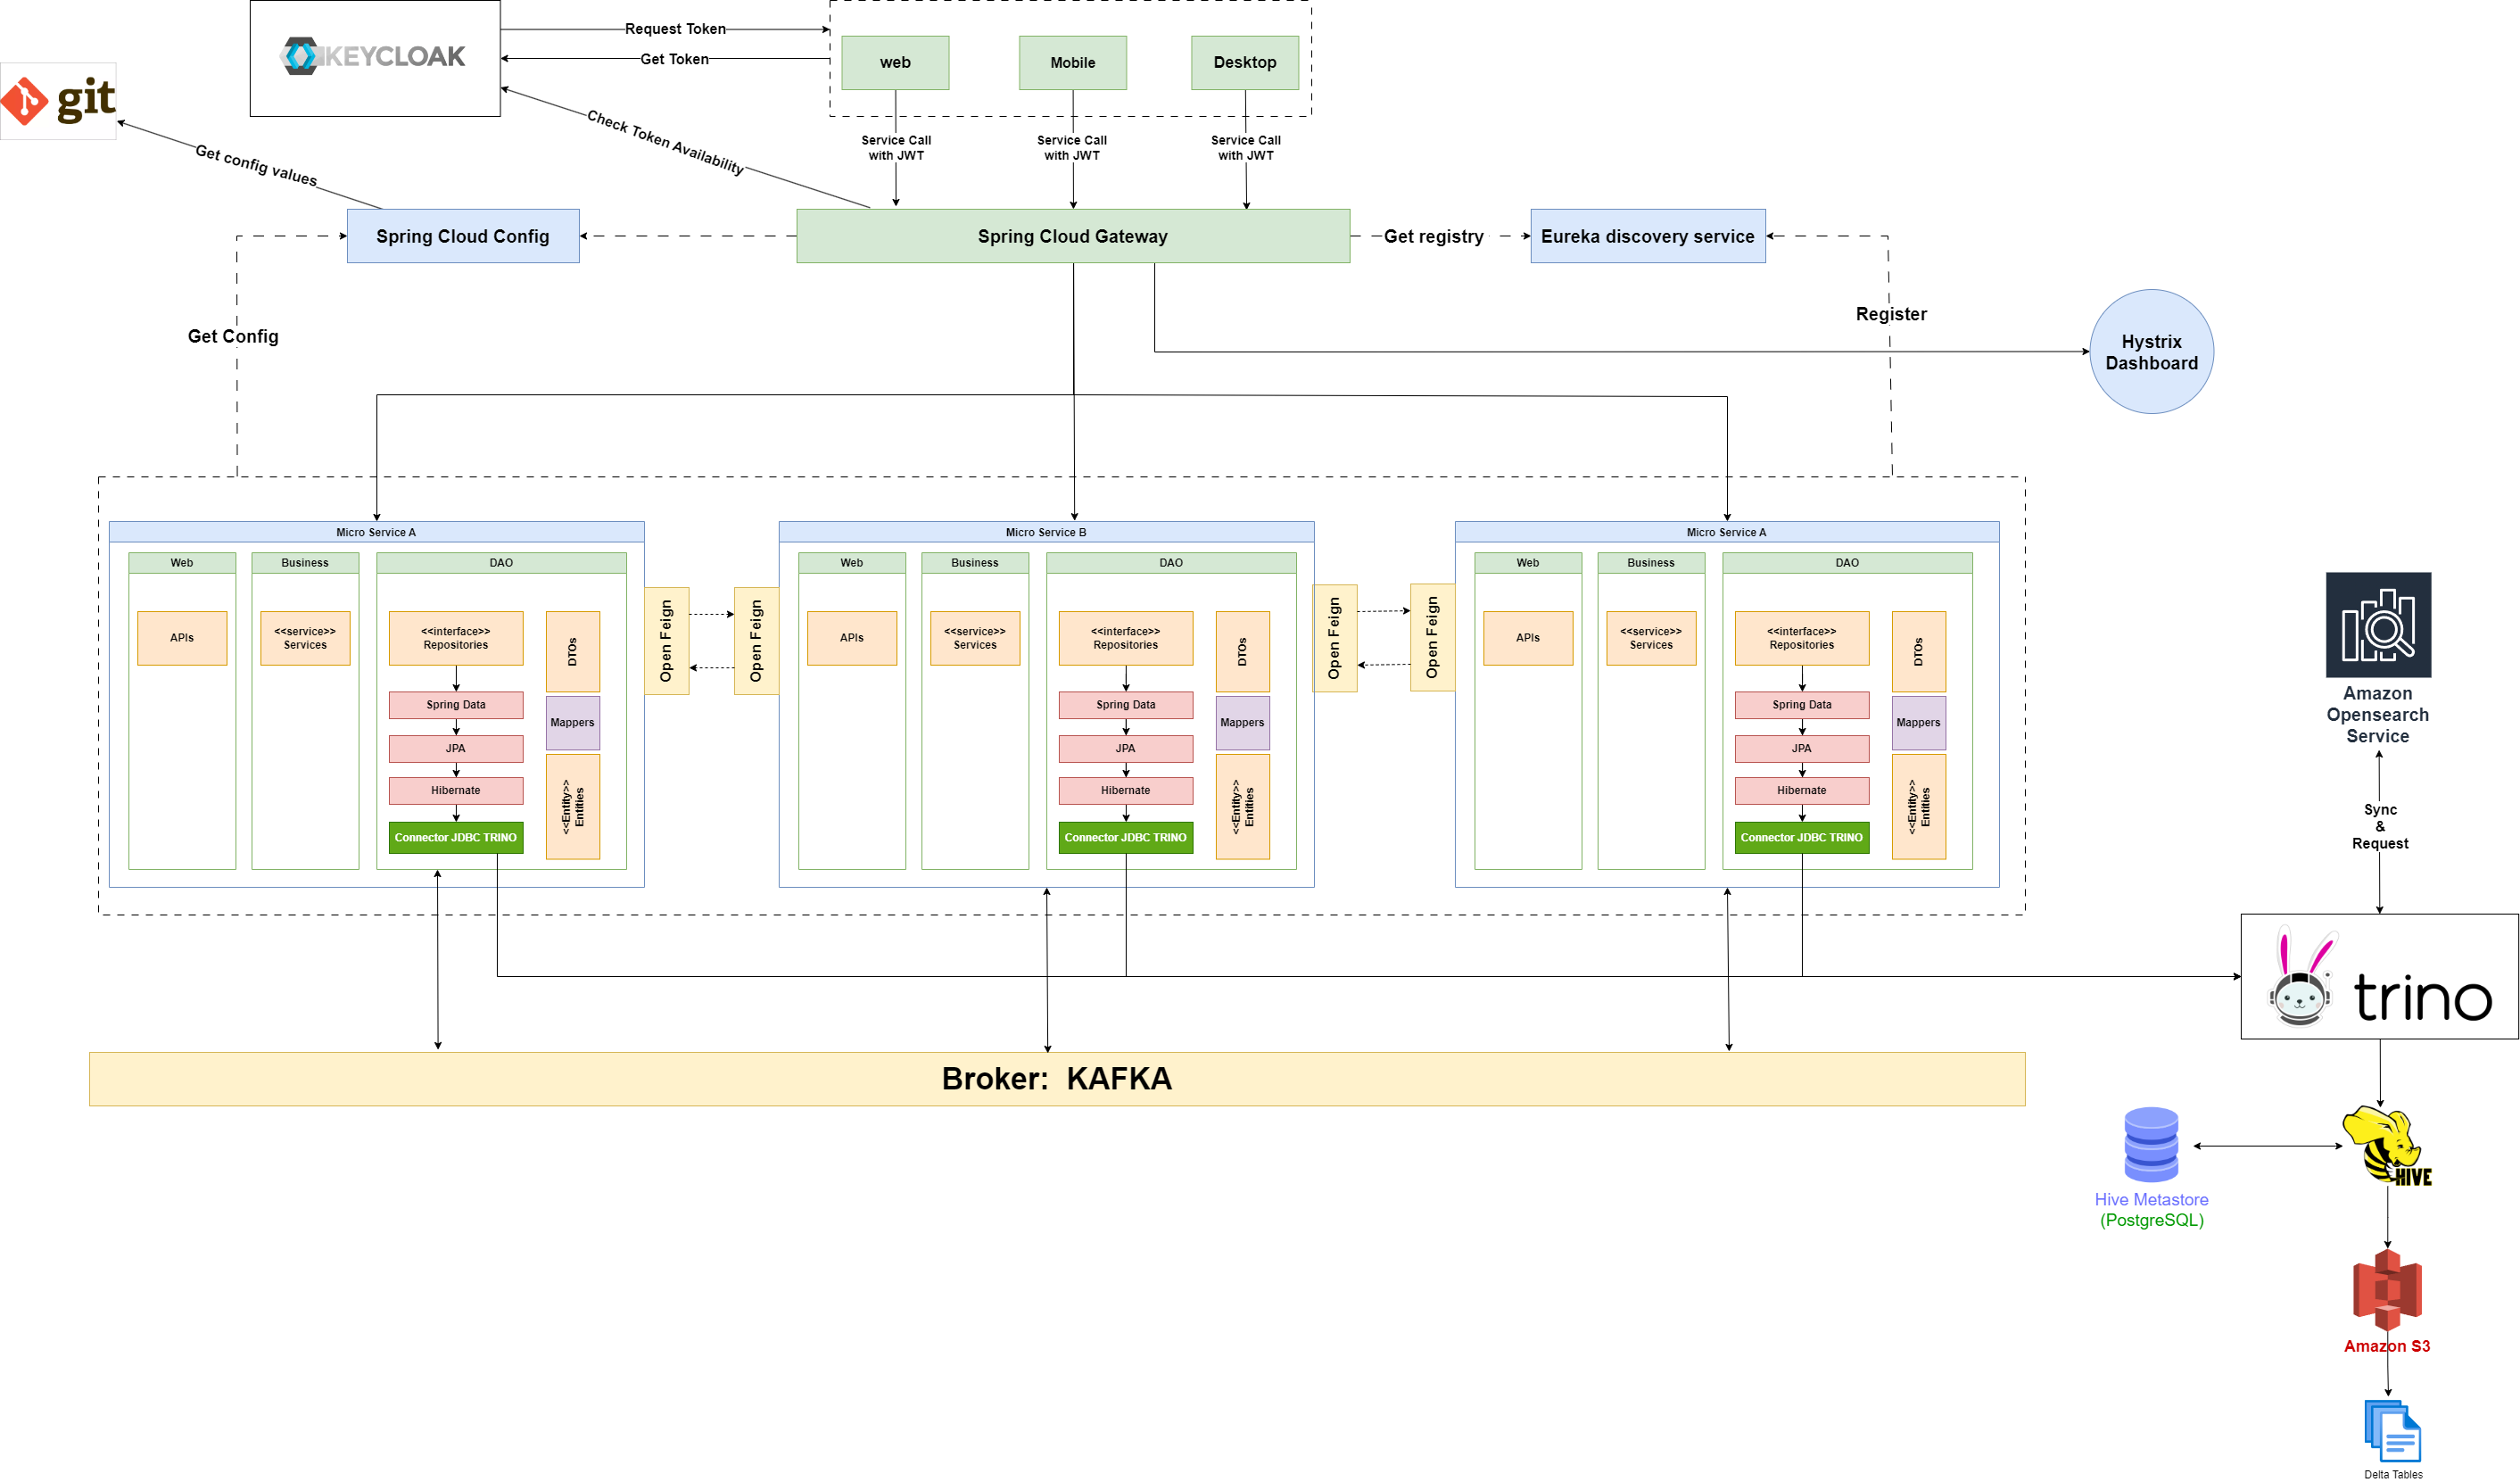
\includegraphics[width=\linewidth]{images/architecture-solution.png}
\caption{Architecture de solution}\label{fig:solution}
\end{figure}

\section{Avantages}

L'architecture que nous avons choisie présente plusieurs avantages significatifs:

\begin{enumerate}
    \item[$\bullet$] \textbf{Évolutivité:} L'architecture basée sur des microservices permet une évolutivité horizontale, ce qui signifie que chaque microservice peut être déployé et mis à l'échelle indépendamment en fonction de ses besoins spécifiques. Cela permet d'ajuster la capacité et les ressources de manière granulaire, ce qui facilite la gestion des charges de travail élevées et l'adaptation aux besoins croissants de l'application.
    \item[$\bullet$] \textbf{Modularité:} La conception modulaire des microservices permet une gestion plus efficace du développement, du déploiement et de la maintenance. Chaque microservice peut être développé indépendamment, ce qui facilite la collaboration entre les équipes et favorise la réutilisation du code. De plus, les modifications ou les mises à jour apportées à un microservice n'ont pas d'impact sur les autres, ce qui réduit les risques d'erreurs et de conflits. 
    \item[$\bullet$] \textbf{Flexibilité technologique:} Les microservices offrent une flexibilité en termes de choix technologiques. Chaque microservice peut être développé en utilisant les technologies les plus adaptées à sa fonctionnalité spécifique. Cela permet d'exploiter au mieux les avantages de chaque technologie et de choisir les outils les mieux adaptés à chaque composant de l'architecture. 
    \item[$\bullet$] \textbf{Communication efficace:} L'utilisation de Kafka comme broker de streaming facilite la communication entre les microservices. Kafka garantit la fiabilité et la scalabilité des échanges d'événements en temps réel, ce qui permet une communication fluide et une synchronisation efficace entre les différents composants du système. 
    \item[$\bullet$] \textbf{Sécurité renforcée:} L'intégration de Keycloak pour l'authentification et l'autorisation offre un niveau élevé de sécurité. Les jetons JWT sont utilisés pour l'identification des utilisateurs, et Spring Cloud Gateway assure la vérification et la gestion de ces jetons. Cela garantit que seules les personnes autorisées ont accès aux ressources et aux fonctionnalités appropriées, renforçant ainsi la sécurité de l'application.
    \item[$\bullet$] \textbf{Performances optimisées:}  L'utilisation de Trino comme moteur de requête distribué permet d'interroger et de traiter de grandes quantités de données de manière parallèle et efficace. Trino offre des performances élevées et une optimisation des requêtes, ce qui permet d'obtenir des résultats plus rapidement et d'améliorer l'expérience utilisateur. 
\end{enumerate}

\section*{Conclusion}
L'étude de faisabilité des connecteurs pour manipuler Delta Lake nous a permis de prendre des décisions éclairées sur l'implémentation de la solution. Bien que Spark soit largement utilisé et intégré à l'écosystème Big Data, Trino offre des avantages significatifs en termes de flexibilité et de performances pour les requêtes SQL. En fonction de nos besoins spécifiques et des contraintes techniques, nous avons opté pour l'utilisation de Trino comme connecteur pour manipuler Delta Lake dans notre solution.

\else
    \chapter{Izicap}\label{chap:1}
    \minitoc\addcontentsline{toc}{section}{Introduction}
\section{Introduction}
The objective of this section is to present the general context of the project, starting with the host organization, IZICAP, where I completed a 5-month internship. We will describe their activities, strategy, values, as well as the organizational structure and profiles involved in my project. Then, we will address the work request that expresses the functional requirements on which I based the design and implementation of the solution, as well as the methodology followed to achieve the set objectives.

\section{Presentation of the Host Organization}
\subsection{IZICAP}
IZICAP is a unique and innovative company focused on data analysis, loyalty, and digital marketing for small and medium-sized enterprises (SMEs). Their user-friendly and easy-to-install solution is based on the SaaS model, allowing for the utilization of customers' transactional data from payment cards.

By collaborating with banks and acquirers, IZICAP offers an enhanced value proposition and provides a powerful digital marketing tool to SMEs. Their mission is to support merchants on a daily basis to accelerate the development of their businesses, thereby addressing their specific needs.

IZICAP's story dates back to 2013 when it emerged in an ever-evolving and increasingly complex landscape of financial services. Since then, traditional banking and payment models have been continually threatened by new, more innovative challenger companies. Intense competition means that merchant loyalty can no longer be taken for granted, and often acquirers and payment service providers are compelled to reduce their fees.

After establishing a strong presence in France through partnerships with Groupe BPCE and Crédit Agricole, Izicap formed a partnership with Nexi, the leading acquirer and fintech in Italy, and joined Mastercard's StartPath program with the aim of significantly expanding its global reach. This strategic expansion strengthens their position in the market and confirms their commitment to offering their services to a wider audience.

With Izicap, SMEs have access to an innovative solution that leverages data analysis to optimize their loyalty and marketing strategy. With their expertise and growing international presence, IZICAP is determined to support business growth and help them thrive in an ever-changing commercial environment.
\subsection{Strategic Partnerships}
IZICAP has established strategic partnerships with several key players in the financial industry. Among their notable partners are:
\begin{itemize}
\item \textbf{Groupe BPCE:} Izicap collaborated with Groupe BPCE, one of the leading banking groups in France, to provide their loyalty and digital marketing solution to merchants.
\item \textbf{Crédit Agricole:} Izicap partnered with Crédit Agricole, one of the largest French banks, to offer their services to merchants within their network.
\item \textbf{Nexi:} Izicap formed a partnership with Nexi, the leading acquirer and fintech company in Italy. This collaboration allows Izicap to expand its presence in the Italian market and benefit from Nexi's expertise in the field of payment services.
\item \textbf{Mastercard StartPath:} Izicap joined Mastercard's StartPath program, which supports startups and innovative companies in the fintech field. This collaboration provides Izicap with an opportunity to increase its visibility and expand internationally.
\item \textbf{BBVA:} Izicap also established a partnership with BBVA, one of the major banks in Spain and Latin America. This collaboration with BBVA strengthens Izicap's presence in the Spanish market and enables the company to offer its loyalty and digital marketing solutions to merchants affiliated with BBVA. The partnership with BBVA demonstrates Izicap's commitment to expanding its reach and working with major players in the financial industry to support small and medium-sized enterprises in their growth.
\item \textbf{Ingenico:} Izicap partnered with Ingenico, one of the leading providers of payment solutions and merchant services globally. Through this partnership, Izicap is able to integrate its loyalty and digital marketing solution into Ingenico's payment terminals, providing a comprehensive solution to merchants using Ingenico's services. This collaboration strengthens Izicap's position as a provider of innovative loyalty and marketing solutions, leveraging Ingenico's expertise and global reach in the payments industry.
\end{itemize}
\begin{figure}[H]
\centering

\includegraphics[width=\linewidth]{images/partenaires.png}
\caption{Strategic Partnerships}\label{fig:partnerships}
\end{figure}

\section{Organizational Structure}
\begin{figure}[H]
\centering
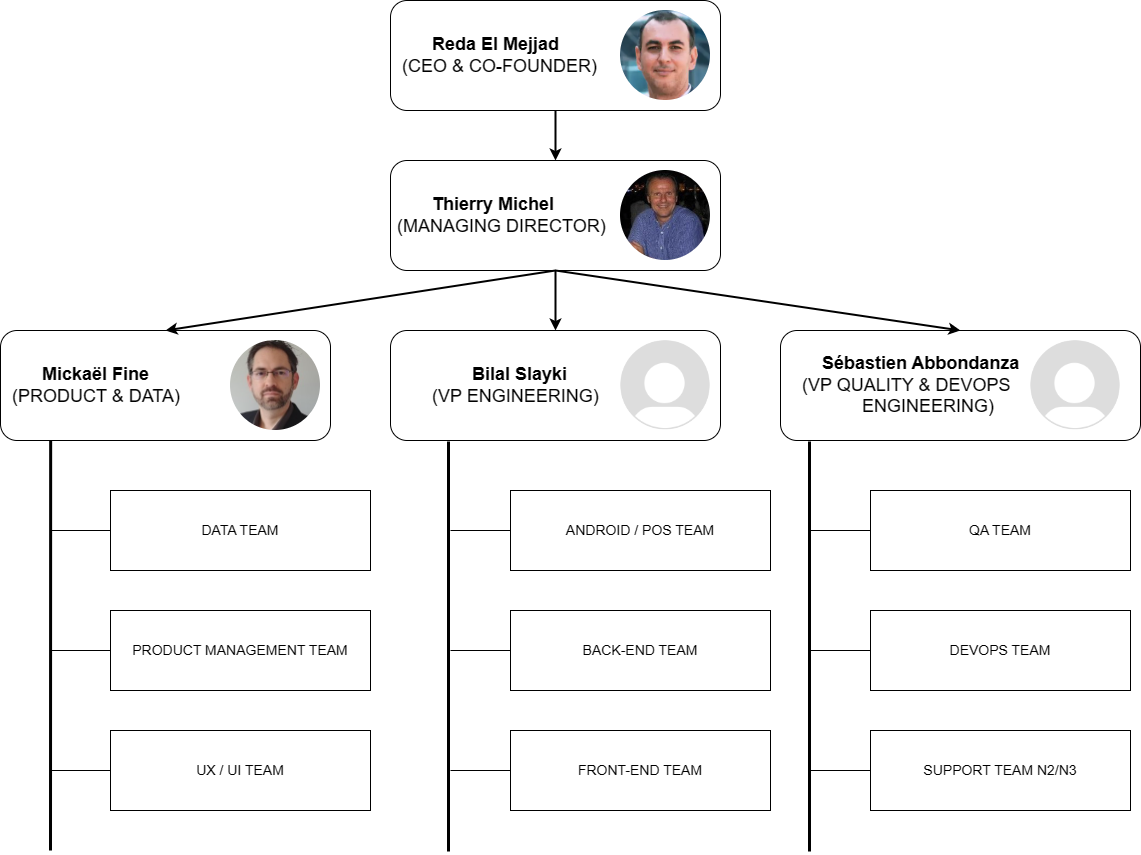
\includegraphics[width=0.75\linewidth]{images/organigram.png}
\caption{IZICAP Organizational Structure}\label{fig:organigram}
\end{figure}

Within the project team, I had the opportunity to work in a versatile manner across different domains. I actively contributed to backend development by participating in the design and implementation of microservices. I also collaborated with the frontend team, bringing my expertise in integrating microfrontends and improving the user experience. Additionally, I was involved in data management, contributing to the implementation of Delta Lake and optimizing data flows. This diverse experience allowed me to gain a holistic view of the project and effectively collaborate with different teams to achieve the set objectives.

\section{Project Framework}

The project involves the revamping of the "Smart data" application, which refers to the process of extracting valuable information from large amounts of data to make informed business decisions.

Smart data allows us to:

\begin{enumerate}
\item \textbf{Data collection}: Izicap helps businesses collect customer data from various touchpoints such as point-of-sale systems, loyalty programs, online interactions, etc. Ensure the integration of their data collection tools into your existing systems or processes.
\item \textbf{Data analysis}: Izicap's smart data solution enables you to analyze the collected data to discover trends, patterns, and customer behaviors. Use their analytics tools and algorithms to gain actionable insights from the data.
\item \textbf{Customer segmentation}: Segment your customer base based on their preferences, purchase history, demographic characteristics, or other relevant criteria. Izicap's smart data solution can assist you in identifying different customer segments and creating personalized marketing strategies for each segment.
\item \textbf{Personalized marketing}: Utilize the insights derived from Izicap's smart data solution to create targeted marketing campaigns. Send personalized offers, promotions, or recommendations to specific customer segments, thereby increasing the chances of conversion and customer satisfaction.
\item \textbf{Customer loyalty}: Leverage Izicap's smart data solution to identify customers who are at risk of churning or no longer making purchases from you. Develop loyalty strategies by offering incentives, loyalty programs, or personalized communications to keep them engaged and loyal to your brand.
\item \textbf{Performance tracking}: Regularly monitor the performance of your marketing campaigns and customer engagement efforts. Izicap's solution can provide you with metrics and reports to evaluate the effectiveness of your strategies and make data-driven adjustments when necessary.
\item \textbf{Continuous improvement}: Smart data solutions are most effective when used iteratively. Regularly analyze data, adapt your strategies, and refine your approach based on new insights and evolving customer behavior.
\end{enumerate}

\begin{figure}[H]
\centering

\includegraphics[width=0.6\linewidth]{images/smart-data-izicap.png}
\caption{Smart data Izicap}\label{fig:smart-data-Izicap}
\end{figure}

\section{System Architecture - Smart Data}

The figure below visualizes the structure and key components of our system, as well as the interactions between them. It forms the foundation of our system and plays a crucial role in providing features and services to our users.

\begin{figure}[H]
\centering
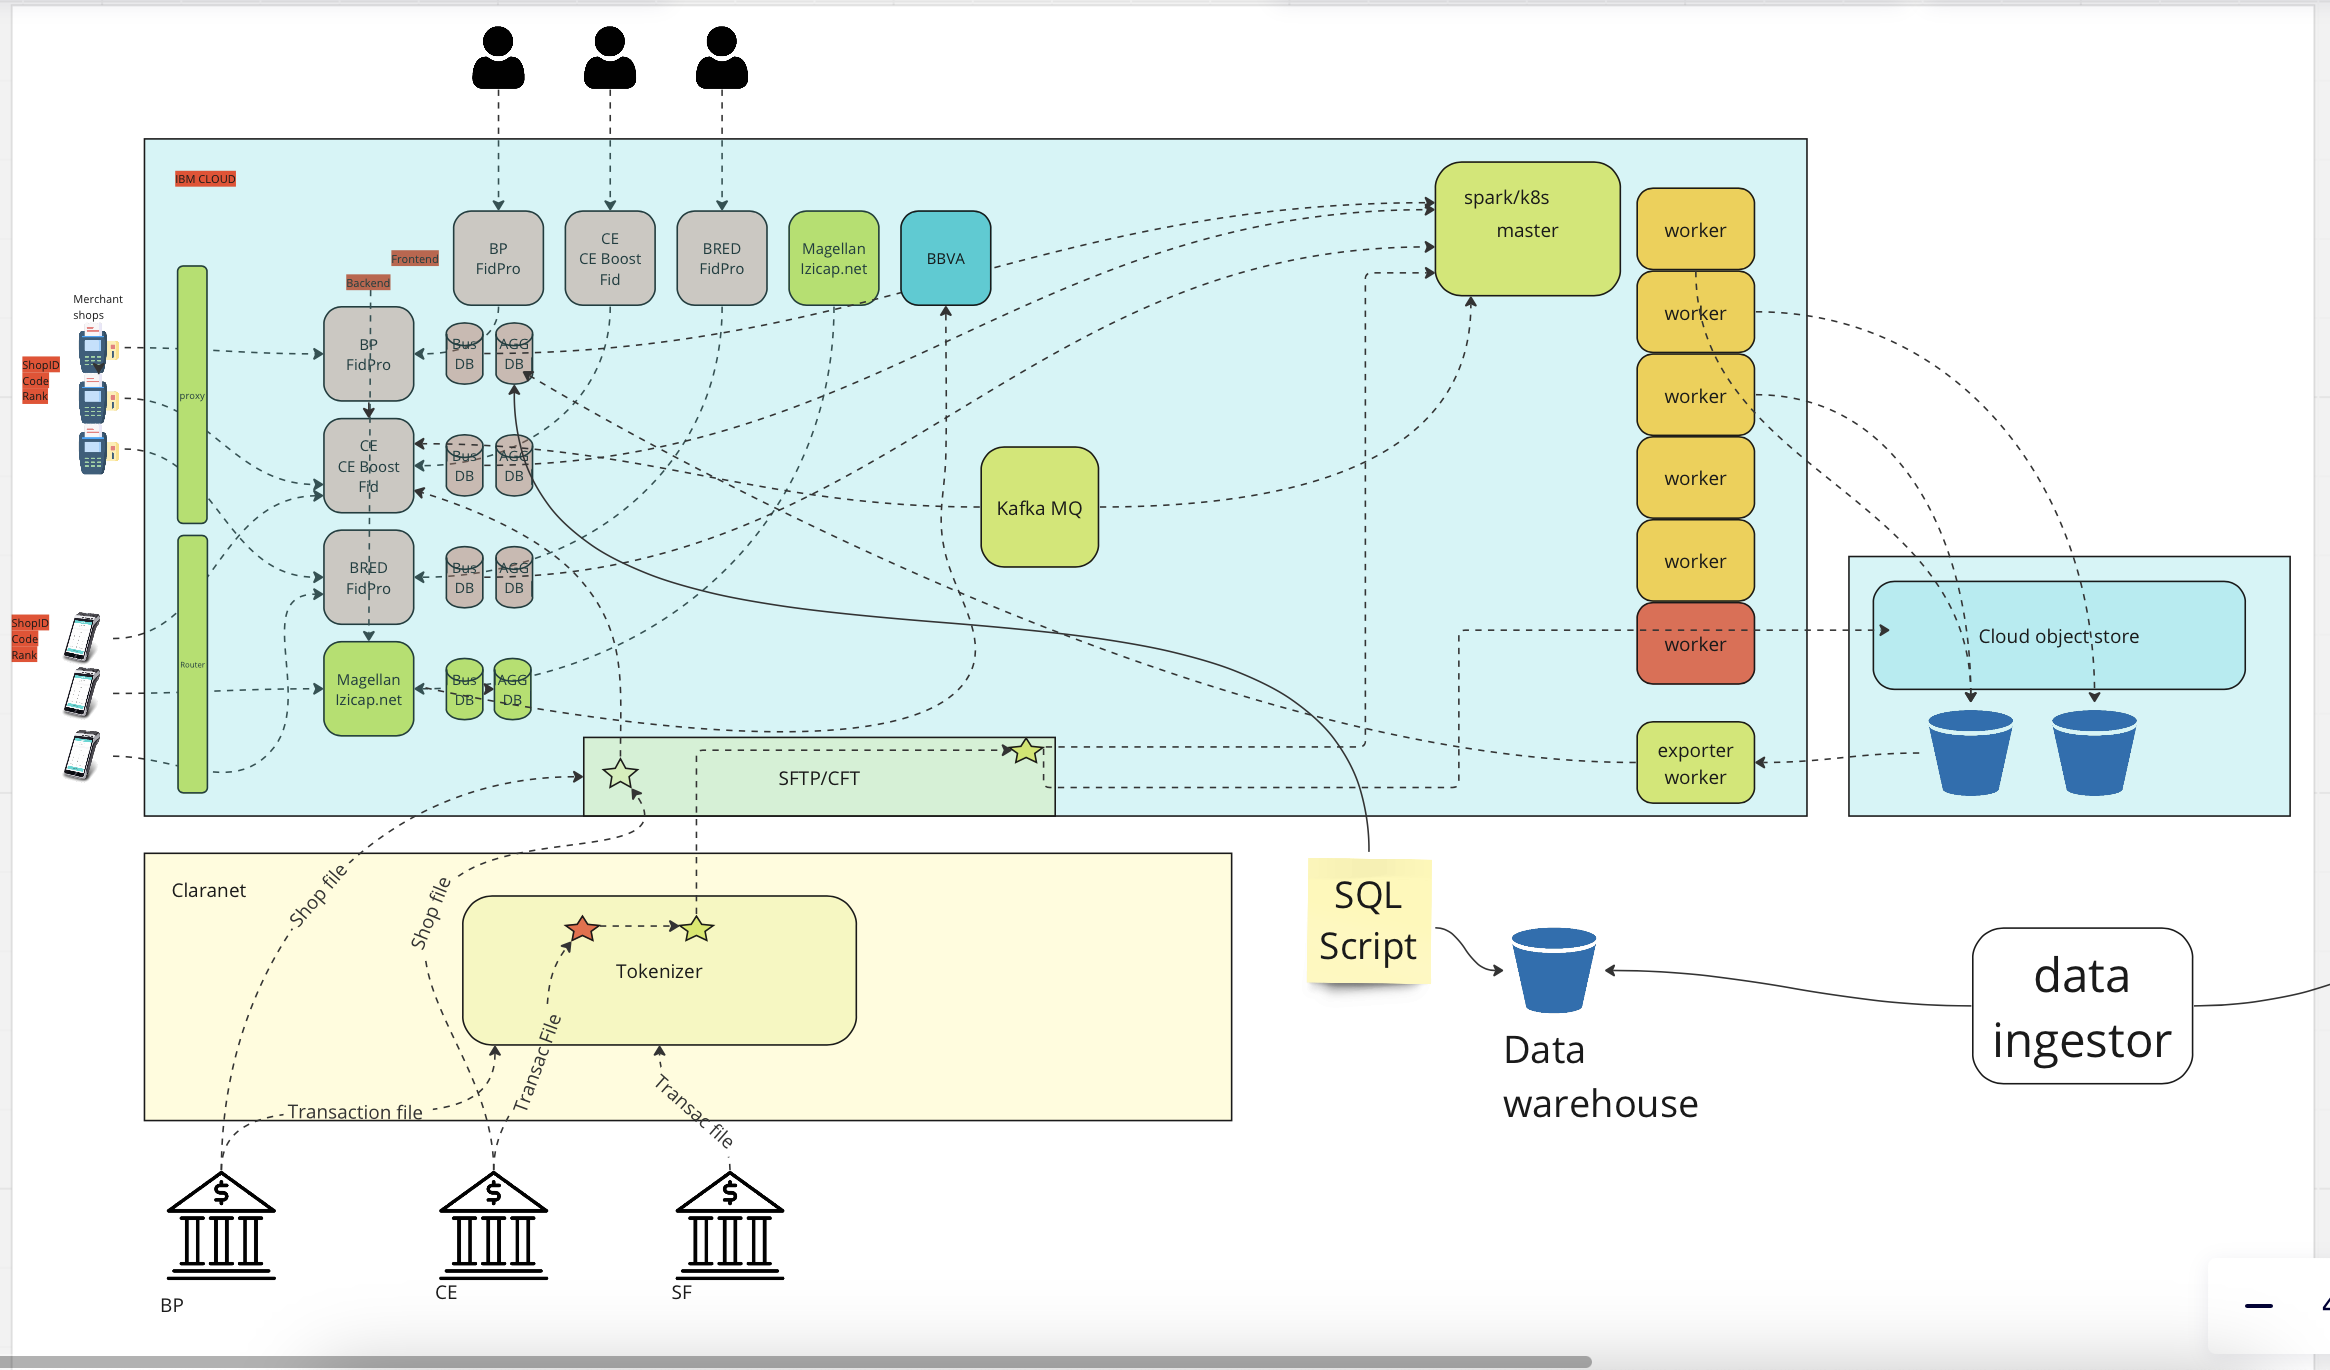
\includegraphics[width=\linewidth]{images/archi-globale.png}
\caption{Current System Architecture}\label{fig:monolithic-architecture}
\end{figure}

This diagram represents the functioning of the current monolithic architecture, which has several disadvantages that can hinder the efficiency, flexibility, and maintainability of the system. Here is a detailed description of the main drawbacks:

\begin{enumerate}
\item \textbf{Complexity and dependencies}: The monolithic architecture involves grouping all modules and functionalities of the system into a single block. This creates strong dependencies between different components, making understanding, management, and updates complex. Changes made to one part of the system can have repercussions on other parts, making testing, deployment, and bug fixing more challenging.
\item \textbf{Limited scalability}: Monolithic architecture often struggles to adapt to increased load or growing demand. Since all components are bundled into a single monolith, it is difficult to selectively scale a specific part of the system. This can lead to bottlenecks, reduced performance, and poor resource allocation when dealing with large data volumes or managing an increase in the number of users.
\item \textbf{Complex deployments and high risks}: With a monolithic architecture, deployments require updating the entire system, even for minor changes. This increases the risks of errors and regressions, as a single mistake can result in the unavailability of the entire system. Additionally, deployments need careful planning and coordination, which can lead to longer downtimes and service interruptions for users.
\item \textbf{Technological choice challenges}: In a monolithic architecture, the technologies used are often tightly coupled and integrated. This can make it difficult to adopt new technologies or integrate specialized components. Upgrading versions or adding new features can be limited by initial technological choices, hindering innovation and adaptation to market changes.
\item \textbf{Cohesion and responsibilities}: Monolithic architecture does not facilitate a clear separation of responsibilities and functionalities. Different modules of the system are often tightly coupled and may share common features. This makes isolating issues, module-specific maintenance, and code reuse specific to a domain challenging.
\end{enumerate}

\section{Problem and Functional Needs}

The problem at hand lies in the currently used monolithic architecture, which presents limitations in terms of scalability, flexibility, and maintainability. The constraints imposed by this architecture make it complex to deploy new functionalities and can potentially disrupt the entire system. Additionally, the use of a traditional relational database such as MariaDB proves insufficient for efficiently handling large volumes of transactional data. It is worth noting that the Smart Data application has been in existence for 10 years and has been developed using the Groovy language. This long period of existence attests to the stability and maturity of our system. However, the use of Groovy may present certain constraints in terms of maintainability and scalability, especially when it comes to integrating new technologies and managing more modern architectures.

\subsection*{Functional Needs}

To address these challenges, different functional needs have been identified:

\begin{enumerate}
\item[$\bullet$] \textbf{Scalability}: It is necessary to have an architecture that can easily adapt to a growing number of users, transactions, and data. It is essential that our system can scale harmoniously and maintain its performance even with a significant increase in workload.
\item[$\bullet$] \textbf{Flexibility}: We need to be able to introduce new functionalities independently and deploy them without disrupting the entire system. An approach based on microservices and microfrontends will enable us to achieve this flexibility by facilitating the development, testing, and isolated deployment of each component.
\item[$\bullet$] \textbf{Improved Performance}: It is crucial to have a data infrastructure capable of efficiently handling large volumes of transactional data. By replacing MariaDB with Delta Lake, we will be able to leverage advanced features such as ACID transaction management and compatibility with powerful analysis tools, significantly improving the performance and reliability of our system.
\item[$\bullet$] \textbf{Separation of Responsibilities}: We aim for better separation of responsibilities between different components of our system. Microservices will allow us to decouple functionalities, assign them to specific teams, and promote more effective code management, simplified maintenance, and increased scalability.
\end{enumerate}

\section{Internship Objectives}

The project falls within the scope of renewing the functionalities of the Smart Data application, aiming to improve its scalability, flexibility, and performance. In this context, the objectives of the internship are as follows:

\begin{enumerate}
\item Study and analyze the current architecture of the SMART DATA application to understand the constraints and limitations that hinder its growth and evolution.
\item Propose and design a migration strategy from the monolithic architecture to an architecture based on microservices and microfrontends, thus enabling better modularity and greater flexibility in the development and deployment of functionalities.
\item Implement multiple microservices with Spring Boot within the new architecture, using appropriate technology and ensuring its seamless integration with other components of the system.
\item Evaluate the benefits and implications of using Delta Lake as a replacement for the MariaDB database, with a focus on performance, transaction management, and integration with analysis tools.
\item Integrate Trino into the architecture to enable the execution of complex SQL queries and optimize data processing, ensuring effective collaboration with the development team.
\item Set up a deployment and management infrastructure for microservices, using tools such as Kubernetes, Docker, and Jenkins, to facilitate deployment, scaling, and component management.
\item Design and implement unit tests and integration tests to ensure the quality and reliability of the new components developed within the microservices-based architecture.
\item Thoroughly document the migration process and the technological choices made, providing clear instructions for the future maintenance of the architecture and management of updates.
\item Collaborate closely with the existing team to facilitate the transition to the new architecture, providing technical support, guidance, and training on the new technologies used.
\end{enumerate}

\section{Project Implementation Process}

The project implementation process followed several iterations called "sprints," typically lasting two weeks each. Each sprint focused on delivering functional increments of the application, enabling quick tangible results.

Here are the key steps of the project implementation process based on the Scrum methodology:

\begin{enumerate}
\item \textbf{Product backlog definition:} In collaboration with stakeholders and the development team, we identified and prioritized the features to be developed and integrated into the microservices-based architecture.
\item \textbf{Sprint planning:} At the beginning of each sprint, we held a planning meeting to define the specific sprint goals, select tasks to be accomplished, and estimate the required effort.
\item \textbf{Iterative development:} The development team worked iteratively on the assigned tasks, focusing on accomplishing the identified features for the current sprint.
\item \textbf{Daily stand-up meetings:} Every day, the team gathered for a brief stand-up meeting to share progress, potential obstacles, and coordinate activities.
\item \textbf{Sprint review:} At the end of each sprint, we conducted a sprint review to showcase the developed features and gather feedback from stakeholders. This allowed us to validate the achieved results and plan for the next steps.
\item \textbf{Sprint retrospective:} After the sprint review, we conducted a retrospective to evaluate the sprint's progress, identify strengths and areas for improvement, and adjust our approach accordingly.
\item \textbf{Subsequent iterations:} The planning, iterative development, sprint review, and retrospective process repeated for each subsequent sprint, enabling incremental progress towards the project's objectives.
\end{enumerate}

\begin{figure}[H]
\centering
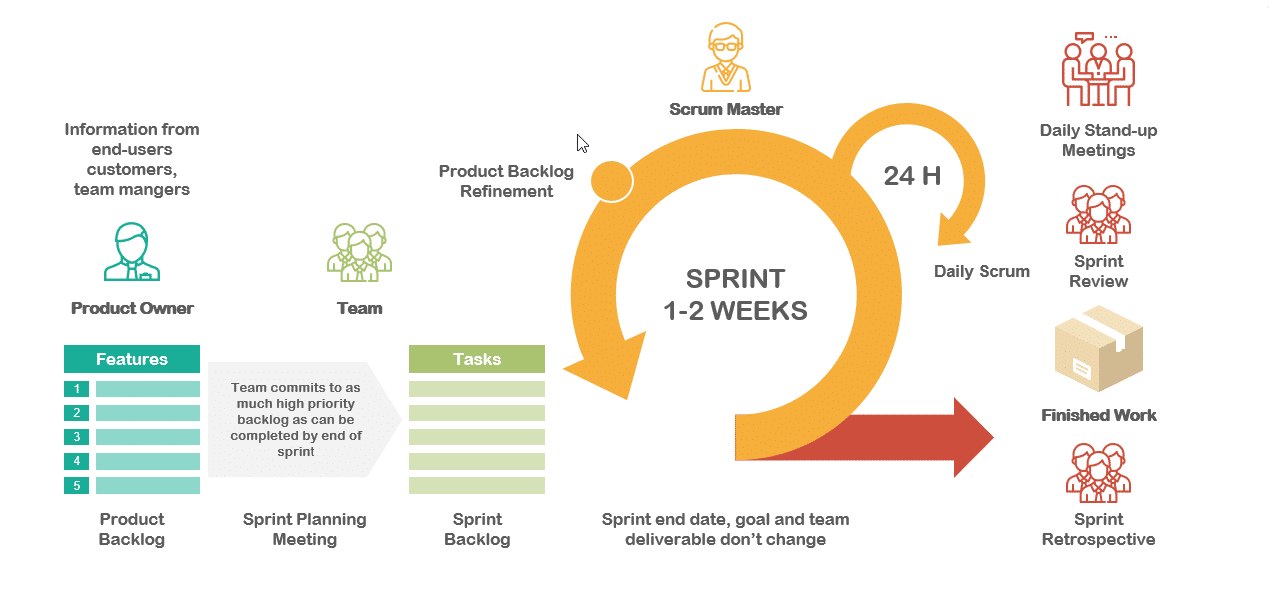
\includegraphics[width=\linewidth]{images/scrum.png}
\caption{Scrum Methodology}\label{fig:scrum}
\end{figure}

\section{Project Planning}
For the project planning, we used the method of modeling the network of task dependencies. This approach allowed us to break down the work into different structured tasks and establish dependency relationships between them.

We also utilized the technique of Gantt chart to graphically represent the project's tasks and resources over time. In the horizontal axis, we listed the different tasks, and in the vertical axis, we defined the days, weeks, or months. Each task was represented by a bar whose length was proportional to the estimated duration of that task.

The Gantt chart enabled us to visualize the distribution of tasks, their duration, and their sequence. Some tasks were performed sequentially, while others could be done in parallel, either partially or entirely. This clear and visual representation helped us plan the project by determining and organizing the different tasks to ensure effective project management.

The following figure presents the Gantt chart detailing the project's planning, with tasks arranged over time and their respective durations. This allowed us to track the project's progress, identify any delays, and take appropriate measures to resolve them.

\begin{figure}[H]
\centering
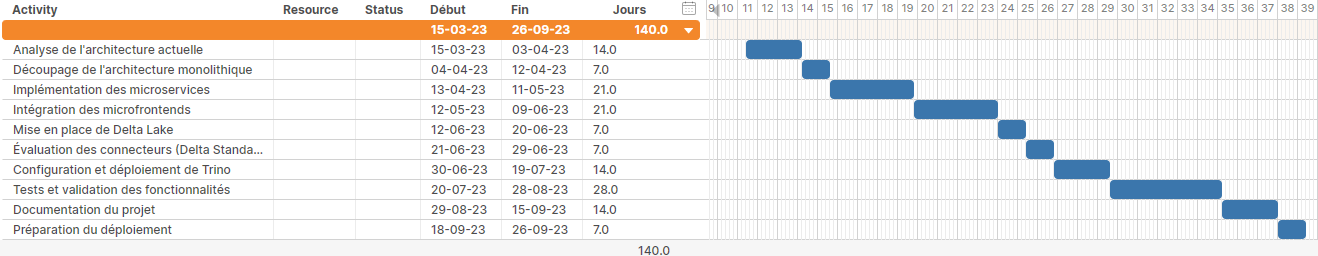
\includegraphics[width=\linewidth]{images/gantt.png}
\caption{Gantt Chart}\label{fig:gantt}
\end{figure}

\addcontentsline{toc}{section}{Conclusion}
\section*{Conclusion}

In conclusion of this section, we have presented the project planning for renewing the functionalities of the SMART DATA application. We developed a schedule based on the modeling of the network of task dependencies, using the technique of the Gantt chart. This chart allowed us to visualize the different activities, their estimated durations, and the required resources.

During the planning, we identified the main project activities, such as the analysis of the current architecture, decomposition of the monolithic architecture, implementation of microservices, integration of microfrontends, implementation of Delta Lake, evaluation of connectors, configuration and deployment of Trino, testing and validation of functionalities, project documentation, deployment preparation, as well as user training and awareness.

We also took into account the total duration of the project, which is estimated to be 5 months, and adjusted the durations of activities accordingly. This provided us with a more precise view of the project's temporal planning.
    
    \chapter{Delta Lake}\label{chap:2}
    \addcontentsline{toc}{section}{Introduction}

\section*{Introduction}

Decision Support encompasses the processes, technologies, and tools used to collect, store, analyze, and present data in order to support decision-making and help businesses gain actionable insights. Decision suuport involves transforming raw data into meaningful information and actionable knowledge for decision-makers. In this chapter, we will explore why we have chosen to adopt Delta Lake instead of its counterparts, as well as microservices and microfrontends.

\section{Difference between a data warehouse, a data lake, a datalakehouse, and Delta Lake}
\begin{enumerate}
\item[$\bullet$] \textbf{Data Warehouse:} A data warehouse is a centralized database specifically designed for reporting and analysis. It stores structured data from different sources, organizes it according to a predefined data model, and optimizes it for analytical queries. Data in a data warehouse is typically consistent, integrated, and historical. However, building and maintaining a data warehouse can be complex and costly.
\item[$\bullet$] \textbf{Data Lake:} A data lake is a centralized data repository that stores large amounts of raw, structured, and unstructured data. Unlike a data warehouse, a data lake does not require prior data modeling. It offers great flexibility and scalability for storing heterogeneous data. However, data integration and data quality can be challenging in a data lake.
\item[$\bullet$] \textbf{Datalakehouse:} Datalakehouse is an emerging architecture that combines the benefits of a data warehouse and a data lake. It enables storing and processing both raw and structured data in a centralized environment. This hybrid approach provides the flexibility of a data lake and the analytical capabilities of a data warehouse. However, implementing a datalakehouse may require additional efforts to ensure data quality and query efficiency.
\item[$\bullet$] \textbf{Delta Lake:} Delta Lake is a technology that integrates with existing data lakes to provide additional features such as ACID (Atomicity, Consistency, Isolation, Durability) transaction management, incremental updates, and data consistency guarantees. Delta Lake is built on Apache Parquet and Apache Arrow, which accelerate analytical queries and improve overall performance. However, using Delta Lake may require additional technical skills and may impact the complexity of the data architecture.
\end{enumerate}

% \subsection{Advantages and disadvantages of each architecture}

\subsection{Data Warehouse}
\textbf{Advantages:}
\begin{enumerate}
\item Consistent and integrated data
\item Predefined data modeling for optimized analysis
\item High performance for analytical queries
\end{enumerate}

\textbf{Disadvantages:}
\begin{enumerate}
\item High construction and maintenance costs
\item Complexity of data modeling
\item Limitations for integrating unstructured data
\end{enumerate}

\subsection{Data Lake}
\textbf{Advantages:}
\begin{enumerate}
\item Economical storage of large amounts of data
\item Flexibility to integrate raw and unstructured data
\item Ability to process data from different sources
\end{enumerate}

\textbf{Disadvantages:}
\begin{enumerate}
\item Difficulty in maintaining data quality and governance
\item Need for advanced tools for data analysis and processing
\item Requires technical skills for efficient data exploitation
\end{enumerate}

\subsection{Datalakehouse}
\textbf{Advantages:}
\begin{enumerate}
\item Combines the benefits of a data warehouse and a data lake
\item Flexibility to store and analyze raw and structured data
\item Ability to evolve based on evolving needs
\end{enumerate}

\textbf{Disadvantages:}
\begin{enumerate}
\item Requires additional efforts for data quality
\item Increased complexity of the data architecture
\item Requires technical skills for setup and management
\end{enumerate}

\subsection{Delta Lake (Datalakehouse)}
\textbf{Advantages:}
\begin{enumerate}
\item ACID transaction management for data consistency
\item Support for incremental updates and stream processing
\item High performance for analytical queries
\end{enumerate}

\textbf{Disadvantages:}
\begin{enumerate}
\item Requires specific technical skills
\item Impact on the complexity of the existing data architecture
\item May require adaptations for seamless integration with existing tools

\end{enumerate}

\begin{figure}[H]
\centering
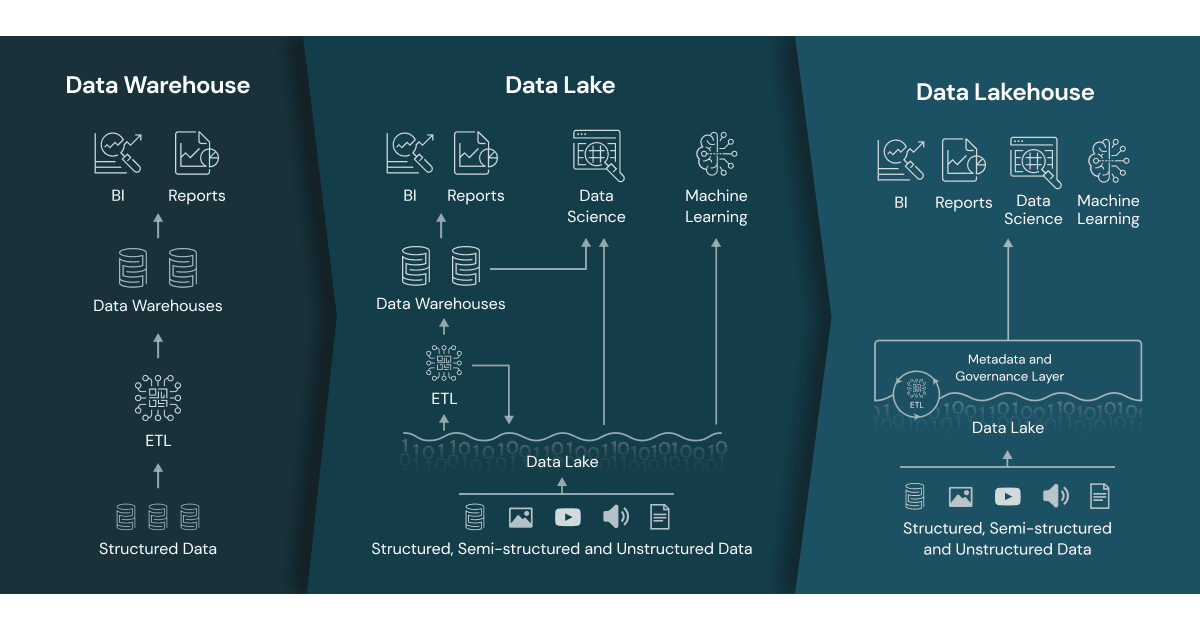
\includegraphics[width=\linewidth]{images/data-warehouse-data-lake-datalakehouse.png}
\caption{Data Warehouse vs Data Lake vs Data Lakehouse}\label{fig:data-warehouse-data-lake-datalakehouse}
\end{figure}

\section{Difference between microservices architecture and monolithic architecture}
\begin{enumerate}
\item[$\bullet$] \textbf{Monolithic:} A monolith is an application that is designed as a single, indivisible entity. All the application's functionalities are grouped together in a single code base, sharing the same resources, databases, and deployments. In a monolithic architecture, there is no clear separation of functionalities into independent services. Any modification or evolution of the application requires changes at a global level.
\item[$\bullet$] \textbf{Microservice:} A microservice is an architectural approach in which an application is built as a set of independent and autonomous services, each focusing on a specific function of the application. Each microservice is developed, deployed, and managed independently, allowing for easier scalability, flexibility, and maintenance. Microservices communicate with each other through well-defined interfaces, typically based on REST APIs or messaging.
\end{enumerate}

\subsection{Advantages and disadvantages of monolithic architecture}
\textbf{Advantages:}
\begin{enumerate}
\item \textbf{Simplicity of initial development:} The monolithic approach allows for rapid development of an application by grouping all functionalities into a single code base. This simplifies dependency management and coordination of different parts of the application.
\item \textbf{Less operational complexity:} With a monolithic architecture, there are fewer components and services to manage, simplifying deployment, monitoring, and management operations. Everything is bundled within a single deployment, which can be easier to handle for operational teams.
\item \textbf{Faster internal communications:} In a monolithic architecture, communications between different parts of the application are faster as they typically occur through internal method calls. This can be beneficial in terms of performance and reduced latency.
\end{enumerate}

\textbf{Disadvantages:}
\begin{enumerate}
\item \textbf{Difficulty in scaling and maintaining:} With a monolithic architecture, scaling and updates can be more complex since every change needs to be made to the entire application. This can slow down the development process and pose risks of errors during deployments.
\item \textbf{Technological rigidity:} A monolithic architecture can result in technological rigidity as all parts of the application must use the same technologies and programming languages. This can limit the opportunities to adopt new technologies or independently evolve specific parts of the application.
\item \textbf{Difficulty in isolating issues:} In case of issues or bugs, it can be more challenging to isolate and resolve them in a monolithic architecture. Since all functionalities are grouped in a single code base, pinpointing the exact origin of the problem can be complex.
\item \textbf{Less flexibility in terms of scalability:} Monolithic architecture can pose challenges in terms of scalability. If a part of the application requires more resources to handle high load, adjusting that specific part without increasing the overall resources of the application can be difficult.
\end{enumerate}

\subsection{Advantages and disadvantages of microservices architecture}
\textbf{Advantages:}
\begin{enumerate}
\item \textbf{Scalability and evolvability:} Microservices allow breaking down the application into several autonomous and independent services, facilitating horizontal scalability. Each microservice can be deployed, scaled, and updated independently, efficiently managing load variations and ensuring easy scalability according to business needs.
\item \textbf{Technological flexibility:} Microservices offer the ability to use different technologies and programming languages for each service. In our case, using Spring Boot allows us to leverage its rich ecosystem and advanced features for rapid application development. It also enables adopting specific technologies based on the needs of each microservice, promoting technological flexibility.
\item \textbf{Independence and autonomy:} Each microservice is designed to operate autonomously, allowing better isolation of functionalities and responsibilities. This facilitates maintenance, testing, and independent deployment of services, reducing the risks of impacting the entire system in case of changes or issues.
\item \textbf{Rapid development and deployment:} Microservices enable an agile development approach by emphasizing shorter development cycles. Teams can focus on specific features and develop them independently, accelerating the overall system development. Additionally, microservices can be continuously deployed through the use of automated deployment techniques, facilitating frequent and rapid updates.
\item \textbf{Ease of maintenance and debugging:} Due to their modular nature, microservices facilitate system maintenance and debugging. In case of problems or errors, it's easier to identify the specific service involved and resolve the issue without impacting the entire system.
\end{enumerate}

\textbf{Disadvantages:}
\begin{enumerate}
\item \textbf{Complexity in managing communications:} Microservices involve communication between different services, typically through REST APIs or messaging. Managing these communications can become complex, especially when numerous services are involved. Issues such as latency, data consistency, and error handling may arise.
\item \textbf{Increased initial development overhead:} Developing microservices requires additional effort to properly decompose functionalities, define interfaces, and set up appropriate infrastructure for service deployment and communication. This can increase the initial workload and require specific skills in distributed architecture.
\item \textbf{Managing data consistency:} With microservices, each service can have its own database or data storage. This can make managing data consistency more complex, particularly when simultaneous updates involving multiple services occur. Techniques such as distributed transactions or asynchronous events may be required to maintain data consistency.
\item \textbf{Deployment and management of multiple services:} With microservices, there is an increased number of services to deploy, manage, and monitor. This may require additional skills in automated deployments, container management, or cluster management. Monitoring the performance and behavior of each service can also become more complex.
\item \textbf{Infrastructure cost:} Microservices may require more complex infrastructure and additional resources to operate effectively. Each service needs to be deployed and run independently, which can result in increased costs related to computing resources and infrastructure management.
\end{enumerate}

\begin{figure}[H]
\centering
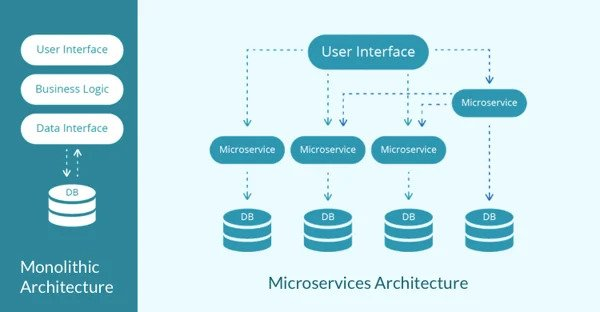
\includegraphics[width=0.6\linewidth]{images/monolithicvsmicroservice.jpg}
\caption{Monolithic Architecture vs Microservices Architecture}\label{fig:monolithicvsmicroservice}
\end{figure}

\section{Difference between microfrontends architecture and monolithic frontend architecture}
\begin{enumerate}
\item[$\bullet$] \textbf{Monolithic Frontend:} A monolithic frontend architecture is an architectural approach where the frontend application is developed as a single entity, typically using a specific framework such as AngularJS. All the features, views, and user interface logic are grouped together in a single code base.
\item[$\bullet$] \textbf{Microfrontends:} Microfrontends are an architectural approach where a frontend application is divided into multiple independent micro-applications, each responsible for a specific part of the user interface. Each micro-application can be developed, deployed, and evolved independently, using different frameworks, languages, and technologies.
\end{enumerate}

\subsection{Advantages and disadvantages of monolithic frontend architecture}
\textbf{Advantages:}
\begin{enumerate}
\item \textbf{Simplicity of initial development:} The monolithic architecture with AngularJS provides a straightforward approach for the initial development of the frontend application. All the features are grouped together in a single code base, making it easier to coordinate and manage the development.
\item \textbf{Ease of communication between components:} In a monolithic architecture, AngularJS components can communicate with each other easily through the AngularJS directives and services system. This allows for quick and efficient communication between different parts of the application.
\item \textbf{Interoperability of features:} Since all the features are developed using AngularJS, it is easier to share features and modules between different parts of the application. This promotes code reuse and simplifies maintenance.
\end{enumerate}

\textbf{Disadvantages:}
\begin{enumerate}
\item \textbf{Difficulty in maintenance and scalability:} As the frontend application becomes more complex, maintaining and evolving the monolithic architecture with AngularJS can become challenging. Changes to one part of the application can have implications on the entire code base, making the development process slower and riskier.
\item \textbf{Performance limitations:} In a monolithic architecture, all the features are loaded together, which can lead to performance issues if the application becomes large. Loading times can be longer, and the application may be less responsive for the user.
\item \textbf{Limited flexibility:} The monolithic architecture with AngularJS can limit technological flexibility. Since all parts of the application are developed using AngularJS, it can be difficult to introduce new technologies or independently evolve specific parts of the application.
\end{enumerate}

\subsection{Advantages and disadvantages of microfrontends architecture}
\textbf{Advantages:}
\begin{enumerate}
\item \textbf{Independence of development teams:} Each micro-application can be developed by a separate team, promoting greater autonomy and better collaboration among development teams. Each team can choose the technologies that best suit their needs.
\item \textbf{Scalability and ease of maintenance:} Microfrontends architecture allows for independent scaling and maintenance of different parts of the application. Changes to one micro-application do not impact others, making maintenance easier and enabling rapid deployment of new features.
\item \textbf{Technological flexibility:} Each micro-application can use the technology, framework, or programming language that best suits its specific domain. This allows for the introduction of new technologies and leveraging the benefits of the latest developments in software engineering.
\end{enumerate}

\textbf{Disadvantages:}
\begin{enumerate}
\item \textbf{Increased complexity:} Microfrontends architecture introduces some complexity in the development and deployment of the application. Managing interactions and communication between different micro-applications may require additional planning and coordination.
\item \textbf{Higher initial development cost:} Developing a microfrontends architecture may require a higher initial investment in terms of resources and time. Developing multiple separate micro-applications and setting up the necessary infrastructure can be more costly than developing a monolithic application.
\item \textbf{Network overhead:} Using microfrontends architecture can result in increased network overhead as each micro-application requires separate requests and resource loading. This can impact application performance and require efficient network management.
\end{enumerate}

\begin{figure}[H]
\centering
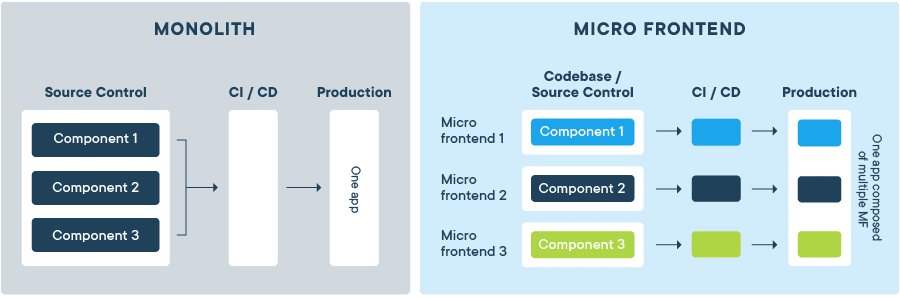
\includegraphics[width=\linewidth]{images/micro-frontend-vs-monolith-frontend.png}
\caption{Monolithic Frontend Architecture vs Microfrontends Architecture}\label{fig:monolithfrontendvsmicrofrontends}
\end{figure}

\section{Solution approach}
\subsection{Data part}
In the context of our solution, we have chosen to replace the existing exporter worker and MariaDB databases with the use of a data lakehouse architecture. A data lakehouse is a hybrid approach that combines the benefits of a data warehouse and a data lake, providing a more flexible and scalable solution for data management.

\subsection{Backend part}
For the implementation of microservices, we have chosen to use Spring Boot, a popular Java framework for application development. By using Spring Boot, we can create standalone microservices that are independent of each other and can be developed, deployed, and scaled individually. Spring Boot also provides features such as data persistence management, security, and REST API creation, making it easier to develop microservices.

\subsection{Frontend part}
For the implementation of microfrontends, we have primarily chosen to use React. The development team can benefit from the rich and mature React ecosystem, as well as its increasing popularity in the frontend development industry. However, it is also mentioned that Angular can be used later if needed, providing additional flexibility in the choice of technologies.

\section*{Conclusion}
When evaluating different data architectures for Izicap, it is important to understand the specific needs related to the management of bank files, transaction receipts, and aggregation operations.

A data warehouse could have been a viable option, offering structured and optimized data structures for analytical queries. However, the main drawback of a data warehouse lies in its static nature, which requires pre-modeling of data and rigid transformation before loading. This can pose challenges when integrating new file types or evolving aggregation requirements.

On the other hand, a data lake has advantages in terms of cost-effective storage and flexibility to integrate raw and unstructured data. However, maintaining data quality and governance can be more complex, and specific technical skills are required to effectively leverage data from the data lake.

Therefore, Delta Lake was favored due to its ability to meet Izicap's specific needs for managing bank files, transaction receipts, and aggregation operations. It provides the necessary flexibility and performance while maintaining data integrity, making it a solid choice for the company's data architecture.

By adopting a microservices-based approach, Izicap can improve the flexibility, scalability, and maintenance of its frontend application. This will enable the company to better meet the changing needs of its users, facilitate collaboration between development teams, and adopt innovative technologies to deliver an optimal user experience.

Microfrontends offer several advantages for Izicap. Firstly, the modularity inherent in microfrontends allows for the development, deployment, and maintenance of different parts of the user interface independently. This promotes collaboration between development teams and enables rapid and efficient evolution. Each micro-application can be developed using the framework and technologies that best suit its specific needs, providing essential technological flexibility for Izicap.

In contrast, the monolithic approach has limitations in terms of scalability and technological flexibility. Changes made to one part of the application can impact the entire system, making evolutions more complex and risky. Additionally, introducing new technologies or frameworks can be challenging in a monolithic architecture, limiting opportunities for innovation and modernization.
    
    \chapter{Technologies used}\label{chap:3}

    \section*{Introduction}
In this chapter, we will examine in detail the key technologies that are used in our solution to provide advanced features and meet the specific needs of our project. The three main technologies we will cover are Delta Lake, Trino, and Microfrontends.

\section{Delta Lake}

Delta Lake is a data management technology that enables efficient and reliable storage, management, and analysis of massive volumes of data. It is built on a file-based Parquet architecture and offers advanced features such as ACID (Atomicity, Consistency, Isolation, Durability) transaction management and compatibility with popular analytics tools. Delta Lake also ensures data integrity, query consistency, and supports replication and recovery in case of failures.

The concept of a `lakehouse' is made possible by Delta Lake. It is a data architecture that combines the benefits of data warehouses and data lakes, providing a unique and consistent approach to data management. Data is stored in Parquet format in the data lake, enabling continuous and batch processing.
\begin{itemize}
\item \textbf{Enables Lakehouse architecture:} Delta Lake enables a continuous and streamlined data architecture that allows organizations to manage and process massive volumes of data in a continuous and batch manner without the hassle of separately managing and operating streaming, data warehouses, and data lakes.
\item \textbf{Enables intelligent data management for data lakes:} Delta Lake provides efficient and scalable metadata management, which provides insights into massive data volumes in data lakes. With this information, data governance and management tasks can be performed more effectively.
\item \textbf{Schema enforcement for improved data quality:} Since data lakes don't have a defined schema, it becomes easy for bad/incompatible data to enter the data systems. Data quality is improved through automatic schema validation, which validates DataFrame and table compatibility before writes.
\item \textbf{Enables ACID transactions:} Most organizational data architectures involve numerous ETL and ELT movements in and out of data storage, which opens it up to more complexity and failure points. Delta Lake ensures data durability and persistence during ETL and other data operations. Delta Lake captures all data changes during data operations in a transaction log, ensuring data integrity and reliability during data operations.
\end{itemize}

\section{Key Benefits and Features of Delta Lake}
\begin{flushleft}
With Delta Lake, data is stored in an optimized format, such as Parquet, in a data lake. This format enables efficient query processing regardless of the mode of data access, whether it is streaming or batch processing.
\end{flushleft}

\begin{figure}[H]
\centering
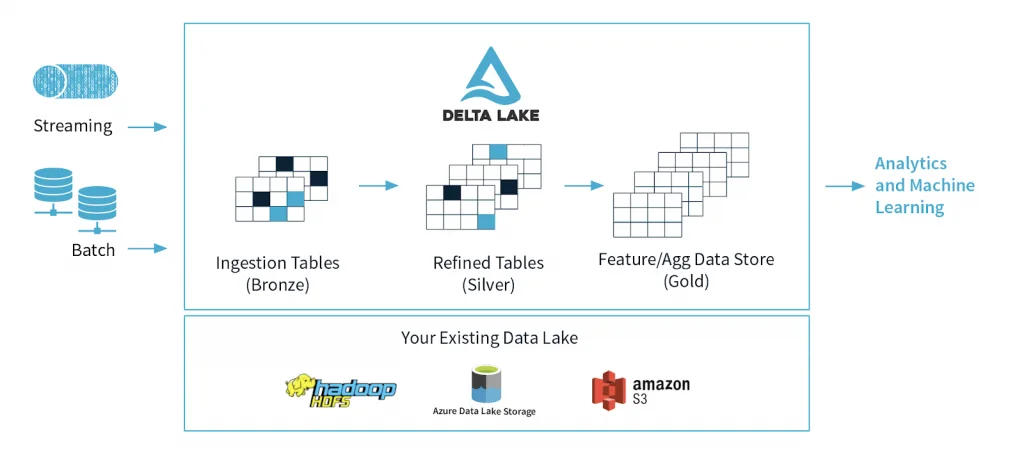
\includegraphics[width=\linewidth]{images/delta_lake_architecture.png}
\caption{Delta Lake multi-hop architecture}\label{fig:delta-lake-architecture}
\end{figure}

\begin{itemize}
\item[\textbullet] \textbf{Audit trails and history:} In Delta Lake, each write exists as a transaction and is sequentially recorded in a transaction log. Therefore, all modifications or validations made to the transaction log are recorded, leaving a complete trail to be used for historical audits, versioning, or time travel purposes. This Delta Lake feature ensures data integrity and reliability for enterprise data operations.
\item[\textbullet] \textbf{Time travel and data versioning:} Since each write creates a new version and stores the old version in the transaction log, users can view/restore old versions of data by providing the timestamp or version number of an existing table or directory to the Spark read API. Using the provided version number, Delta Lake then constructs a complete snapshot of the version with the information provided by the transaction log. Rollbacks and version management play a crucial role in machine learning experimentation, where data scientists iteratively modify hyperparameters to train models and can revert to previous changes if necessary.
\item[\textbullet] \textbf{Unifies batch and stream processing:} Each table in a Delta Lake is both a batch and stream sink. With Structured Streaming in Spark, organizations can efficiently stream and process data. Additionally, with efficient metadata management, scalability, and ACID quality for each transaction, near-real-time analytics becomes possible without using a more complicated two-tier data architecture.
\item[\textbullet] \textbf{Efficient and scalable metadata management:} Delta Lake stores metadata information in the transaction log and leverages the distributed processing power of Spark to quickly process, read, and manage large volumes of data metadata, thereby enhancing data governance.
\item[\textbullet] \textbf{ACID transactions:} Delta Lake ensures that users always see a consistent view of data in a table or directory. It achieves this by capturing every modification made in a transaction log and isolating it at the strongest isolation level, the serializable level. At the serializable level, every existing operation has and follows a serial sequence that, when executed one by one, provides the same result as stated in the table.
\item[\textbullet] \textbf{Data Manipulation Language (DML) operations:} Delta Lake supports DML operations such as updates, deletes, and merges, which play a role in complex data operations such as Change Data Capture (CDC), continuous upserts, and Slowly Changing Dimensions (SCD). Operations like CDC ensure data synchronization across all data systems and minimize time and resources spent on ELT operations. For example, using CDC, instead of ETL-ing all available data, only the recently updated data since the last operation undergoes transformation.
\item[\textbullet] \textbf{Schema enforcement:} Delta Lake performs automatic schema validation by checking a set of rules to determine the compatibility of a DataFrame write to a table. One such rule is the existence of all DataFrame columns in the target table. An occurrence of an extra or missing column in the DataFrame raises an error exception. Another rule is that the DataFrame and the target table must have the same column types, which, if not, triggers an exception. Delta Lake also uses Data Definition Language (DDL) to explicitly add new columns. This data lake feature helps avoid the ingestion of incorrect data, ensuring high data quality.
\item[\textbullet] \textbf{Compatibility with Spark API:} Delta Lake is built on Apache Spark and is fully compatible with the Spark API, enabling the creation of efficient and reliable large-scale data pipelines.
\item[\textbullet] \textbf{Flexibility and integration:} Delta Lake is an open-source storage layer and utilizes the Parquet format for storing data files, which promotes data sharing and facilitates integration with other technologies, fostering innovation.
\end{itemize}

\section{Trino}

Trino, formerly known as Presto, is a distributed, open-source SQL query engine. It is designed to execute interactive and analytical queries at a large scale on heterogeneous and distributed data. Trino offers great versatility by allowing access to various types of data sources, whether they are relational databases, file systems, real-time data sources, or cloud storage services. With its distributed design, Trino enables high performance and horizontal scalability, making it an essential tool for data analysis in our solution.

\begin{figure}[H]
\centering
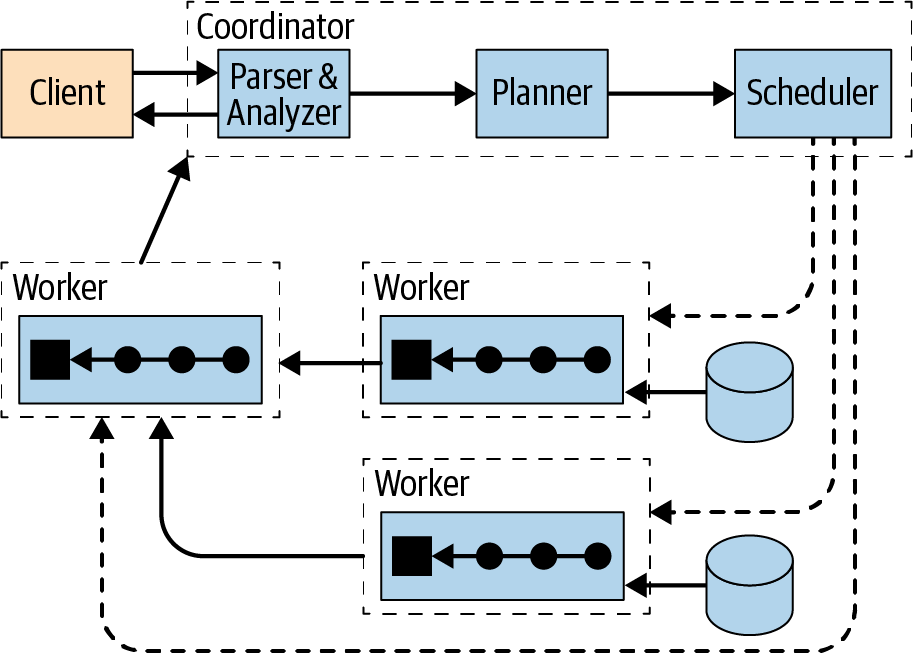
\includegraphics[width=0.8\linewidth]{images/trino_architecture.png}
\caption{Overview of Trino architecture with coordinator and workers}\label{fig:trino-architecture}
\end{figure}

\begin{enumerate}
\item A coordinator is a Trino server that handles incoming queries and manages workers to execute the queries.
\item A worker is a Trino server responsible for executing tasks and processing data.
\item The discovery service typically runs on the coordinator and allows workers to register to participate in the cluster.
\item All communications and data transfers between clients, the coordinator, and workers use REST-based interactions over HTTP/HTTPS.
\end{enumerate}

\section{Spring Boot}

Spring Boot is an open-source framework for Java application development. It provides a simplified and opinionated approach to creating standalone, production-ready Java applications without the need for complex configuration.

One of the main advantages of Spring Boot is its ability to reduce boilerplate configuration and simplify application development by providing smart default configuration definitions and automating many development tasks. It also embeds an application server, making it easy to deploy and run the application without requiring an external application server.

Spring Boot follows the annotation-driven programming paradigm, where annotations are used to configure and orchestrate different parts of the application. It offers a wide range of features, such as dependency injection, externalized configuration, error handling, security, data access, etc. These features are bundled into starters, which are pre-defined dependencies that facilitate adding specific functionality to the application.

With its simplified approach, Spring Boot allows developers to focus more on the business logic of their application rather than tedious configuration tasks. It also promotes good development practices, such as separation of concerns and modularity, making applications more maintainable and scalable.

\section{Keycloak}

Keycloak is an open-source Identity and Access Management (IAM) solution developed by Red Hat. It provides comprehensive features for user management, authentication, authorization, and securing applications.

Keycloak helps centralize and simplify identity management within an IT infrastructure. It offers features such as user registration, multi-factor authentication, role and permission management, session management, and integration with common authentication and authorization protocols like OAuth 2.0 and OpenID Connect.

Keycloak provides functionality for managing roles, administrators, users, and passwords. Here's how Keycloak addresses these aspects:

\begin{enumerate}
\item Keycloak allows defining roles at the realm or application level. Roles can be created and assigned to users to define their permissions and access.
\item Keycloak administrators can create, manage, and assign roles to users through the administration interface or management API.
\item Roles can be used to control access to features, pages, and resources within the application.
\item Keycloak provides specific administration roles like "admin" or "superadmin" that allow users to perform administrative tasks such as managing clients, users, roles, etc.
\item Users can log in using their credentials (username and password) or other supported authentication methods like two-factor authentication, OAuth 2.0, etc.
\item Keycloak supports user-based authentication and provides a registration interface to allow users to create their accounts.
\item Keycloak also offers advanced authentication features such as two-factor authentication, social authentication (via identity providers like Google, Facebook, etc.), and certificate-based authentication.
\end{enumerate}

\section{Kafka}

Kafka is a distributed and scalable data streaming platform designed to efficiently handle the transmission and processing of real-time data streams. It was developed by Apache Software Foundation.

Kafka is based on a distributed log architecture, where data is stored as streams of messages in "topics". Data producers send messages to specific "topics," while consumers subscribe to those "topics" to retrieve the messages. This allows for asynchronous communication and clear separation between data producers and consumers.

The key features of Kafka include:

\begin{enumerate}
\item Scalability: Kafka is designed to handle large volumes of data and can be horizontally scaled to meet growing performance needs. It can handle high workloads and process thousands of messages per second.
\item Fault tolerance: Kafka ensures high availability and fault tolerance by replicating data across multiple nodes in the cluster. This ensures data reliability and availability even in case of node failures.
\item Data durability: Messages stored in Kafka are persistent and can be retained for a defined period. This allows for message replay and data recovery when needed, which is crucial for use cases requiring long-term data retention.
\item Stream processing: Kafka is designed for real-time stream processing. It enables applications to consume continuous data streams and process them in real-time, which is critical for use cases requiring real-time analysis, data pipelines, etc.
\item Integration with other tools: Kafka easily integrates with other tools and frameworks such as Spark, Hadoop, Flink, etc. This enables seamless integration with the Big Data ecosystem and facilitates data ingestion, processing, and streaming.
\end{enumerate}

\begin{figure}[H]
\centering
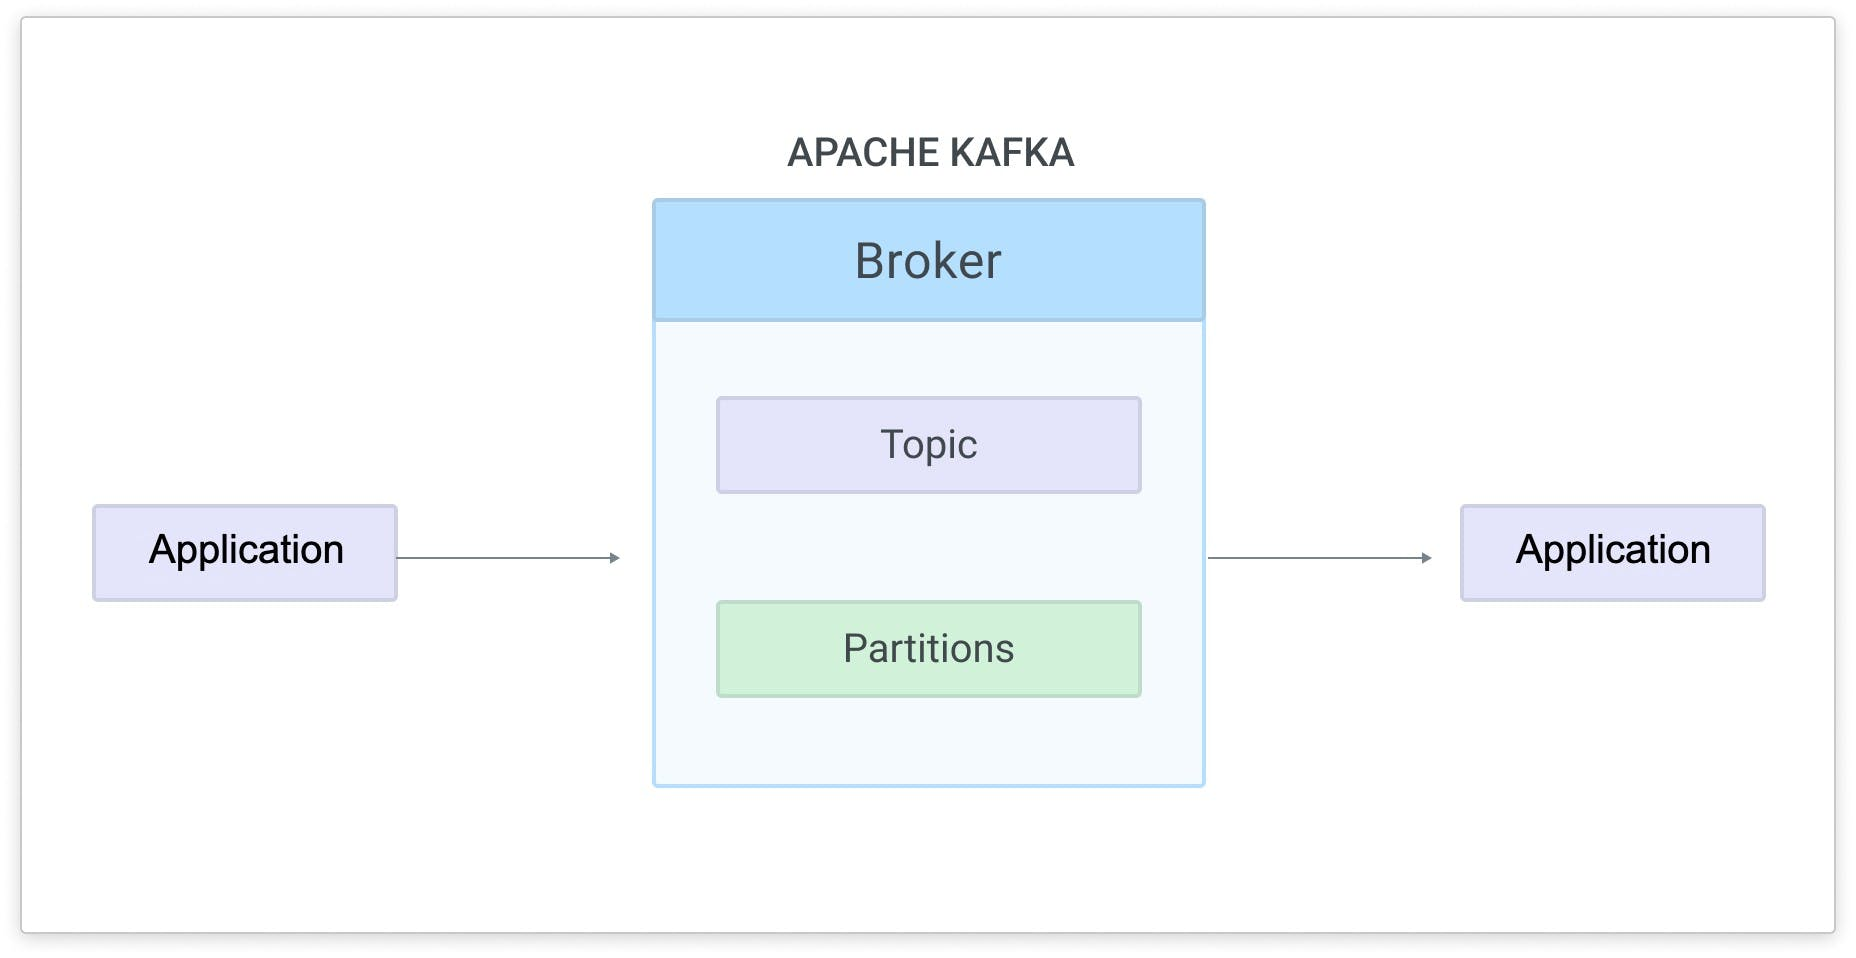
\includegraphics[width=\linewidth]{images/kafka.jpg}
\caption{Kafka Architecture}\label{fig:kafka}
\end{figure}

\section*{Conclusion}
these technologies, developers and data professionals can leverage their strengths to build powerful and scalable applications. Trino enables fast and flexible data querying, Spring Boot simplifies application development, Keycloak provides robust IAM capabilities, and Kafka enables real-time data streaming and processing.
\fi
 
% \include{perspectives}
%%conclusion
\conclusion
Le stage a été une expérience enrichissante qui a permis d'explorer divers aspects des microservices en utilisant des technologies telles que Delta Lake, Trino, Spring Boot, et Keycloak. L'environnement de travail était propice à l'apprentissage et à la mise en pratique de ces concepts.

L'adoption des microservices présente de nombreux avantages par rapport à une architecture monolithique. Les microservices offrent une meilleure scalabilité et flexibilité, permettant le déploiement, le développement et la mise à l'échelle indépendants de chaque service. De plus, la communication entre les microservices via des API facilite l'intégration et la collaboration entre les différentes parties du système.

Pendant le stage, nous avons appris à concevoir et implémenter des microservices en utilisant Spring Boot, en exploitant ses fonctionnalités de persistence, de sécurité, et de création d'API REST. Nous avons également intégré Keycloak pour gérer l'authentification et l'autorisation des utilisateurs dans notre architecture de microservices. L'utilisation de Delta Lake a permis de garantir la fiabilité des données et de faciliter la gestion des mises à jour.
% 
\lhead[]{} \rhead[]{} \chead[]{}

%%biblio
% \addcontentsline{toc}{chapter}{Bibliographie}
% \bibliographystyle{abbrv}
% \bibliography{biblio}


%\chapter*{Annexe}\addcontentsline{toc}{chapter}{Annexe}\label{annexe1}

\subsection*{Étapes clés du déroulement de l'attaque}


Nous allons exploiter quelques failles de ce réseau pour effectuer une attaque man in the middle (MITM).\\

Au début, notre machine Windows peut atteindre normalement le routeur R4.
\begin{figure}[H]
    \centering
    \includegraphics[scale=0.8]{images/ping_b4_1}
    \caption{Ping vers le routeur R4 avec succès}
    \label{fig:ping_b4_1}
\end{figure}
Quand on essaie de tracer le chemin vers R4, on constate que la machine passe par le routeur R1 légitime du lien pour atteindre R4
\begin{figure}[H]
    \centering
    \includegraphics{images/tracert_b4_1}
    \caption{Traces du chemin vers R4}
    \label{fig:tracert_b41}
\end{figure}
L'attaquant sur le lien peut alors passer a l'attaque.
Pour effectuer l'attaque MITM on utilisera l'outil fake\_router6, un utilitaire du package d'outils \textbf{the hacker choice}.
Ainsi sur la machine d'attaque, on active en un premier lieu le forwarding pour être transparent et ne pas bloquer le transit des paquets.
\begin{figure}[H]
    \centering
    \includegraphics{images/attk/fwrd_activation}
    \caption{Activation du forwarding des paquets.}
    \label{fig:activ_fwrd}
\end{figure}
Aussi on lance wireshark pour observer le trafic des paquets sur notre interface dans le réseau.\\
-------\\
Puisque tout est prêt nous allons lancer l'attaque.

\begin{figure}[H]
    \centering
    \includegraphics[scale=0.8]{images/attk/lancement_attk_1}
    \caption{Initialisation de l'attaque}
    \label{fig:attk_init_1}
\end{figure}

L'attaque est en cours et l'attaquant s'annonce comme le routeur par défaut du lien
nous allons maintenant vérifier la table des routes de notre machine windows.
\begin{figure}[H]
    \centering
    \includegraphics{images/attk/tableRoutes_windows}
    \caption{Table des routes de la machine victime}
    \label{fig:win_route_table}
\end{figure}
On constate que l'attaquant s'est insère comme passerelle de la victime.
pour confirmer cela reprenons un tracert vers le routeur r4
\begin{figure}[H]
    \centering
    \includegraphics{images/attk/tracert_b4_2}
    \caption{Chemin vers b4 pendant l'attaque.}
    \label{fig:tracert_b42}
\end{figure}
On peut voir clairement que la victime passe par l'attaquant pour atteindre le routeur.\\

A présent nous allons essayer de capturer une information envoyée par la victime.
Pour cela la victime fait un telnet sur le router R4 pour s'y connecter avec les paramètres suivants:\\
password1:\textbf{cisco}\\
password2:\textbf{class}
\begin{figure}[H]
    \centering
    \includegraphics{images/attk/telnet_r4}
    \caption{Connexion telnet au routeur.}
    \label{fig:telnetr4}
\end{figure}

Une fois la connexion réussie, nous allons voir avec wireshark les paquets de connexion et y retrouver les paramètres de connexion.
\begin{figure}[H]
    \centering
    \includegraphics[width=1.0\textwidth]{images/attk/c}
    \includegraphics[width=1.0\textwidth]{images/attk/i}
    \includegraphics[width=1.0\textwidth]{images/attk/s}
    \includegraphics[width=1.0\textwidth]{images/attk/c2}
    \includegraphics[width=1.0\textwidth]{images/attk/o}   
    \caption{Premier paramètre de connexion au routeur R4: \textbf{c-i-s-c-o}}
    \label{fig:param_conn_r4}
\end{figure}
\begin{figure}[H]
    \centering
    \includegraphics[width=1.0\textwidth]{images/attk/param2_c}
    \includegraphics[width=1.0\textwidth]{images/attk/param2_l}
    \includegraphics[width=1.0\textwidth]{images/attk/param2_a}
    \includegraphics[width=1.0\textwidth]{images/attk/param2_s1}
    \includegraphics[width=1.0\textwidth]{images/attk/param2_s2}
    \caption{Second paramètre de connexion au routeur R4: \textbf{c-l-a-s-s}}
    \label{fig:param_conn2}
\end{figure}
Les paramètres on été retrouves donc l'attaque a été un succès!

%\subsection*{Mitigations}
%Pour sécuriser ce réseau afin d'éviter ce genre d'attaque, deux mesures de sécurité peuvent être configurées.
%\begin{itemize}
%    \item le SEND
%    \item le RaGuard
%\end{itemize}





\end{document}          
